
\documentclass{article}[12pt]

\usepackage[utf8]{inputenc}
\usepackage{amsmath}
\usepackage{amsfonts}
\usepackage{amssymb}
\usepackage{amsthm}
\usepackage{hyperref}
\usepackage{tikz}
\usepackage{graphicx}
\usepackage{cleveref}
\usepackage{natbib}
\usepackage{enumitem}
\usepackage{booktabs}
\usepackage{multirow}
\usepackage{multicol}
\usepackage{array}
\usepackage{float}

%%%
\hypersetup{
	colorlinks=true,
	linkcolor=black,
	citecolor=black}

%%% TIKZ graphics
\usetikzlibrary{positioning, calc, shapes.geometric, shapes.multipart, shapes, arrows.meta, arrows, 	decorations.markings, external, trees}

\tikzstyle{Arrow} = [
thick,
decoration={
	markings,
	mark=at position 0.99 with {  % fix bug with tikz arrow head interference with decoration
		\arrow[thick]{latex}
	}
},
shorten >= 3pt, preaction = {decorate}
]
\tikzstyle{BiArrow} = [
thick,
decoration={
	markings,
	mark=at position 0.99 with {  % fix bug with tikz arrow head interference with decoration
		\arrow[thick]{latex}
	}
},
shorten >= 3pt, preaction = {decorate}
]
\tikzstyle{RedArrow} = [
red, 
line width = 0.5mm,
decoration={
	markings,
	mark=at position 0.99 with {
		\arrow[line width = 0.5mm,red]{latex}
	}
},
shorten >= 3pt, preaction = {decorate}
]

\tikzstyle{BlueArrow} = [
blue, 
line width = 0.5mm,
decoration={
	markings,
	mark=at position 0.99 with {
		\arrow[line width = 0.5mm,blue]{latex}
	}
},
shorten >= 3pt, preaction = {decorate}
]

\tikzstyle{Dashed} = [
thick,dashed,
decoration={
	markings,
	mark=at position 0.99 with {  % fix bug with tikz arrow head interference with decoration
		\arrow[thick]{latex}
	}
},
shorten >= 3pt, preaction = {decorate}
]

\tikzset{
    BiArrow/.style={
        thick,
        decoration={
            markings,
            mark=at position 0.99 with {
                \arrow[thick]{latex}
            },
            mark=at position 0 with {
                \arrow[thick]{latex}
            }
        },
        shorten >= 3pt,
        preaction = {decorate}
    }
}



\newtheorem{remark}{Remark}
\AfterEndEnvironment{remark}{\noindent\ignorespaces}
\newtheorem{assumption}{Assumption}
\AfterEndEnvironment{assumption}{\noindent\ignorespaces}
\newtheorem{proposition}{Proposition}
\AfterEndEnvironment{proposition}{\noindent\ignorespaces}
\newtheorem{theorem}{Theorem}
\AfterEndEnvironment{theorem}{\noindent\ignorespaces}
\newtheorem{corollary}{Corollary}
\AfterEndEnvironment{corollary}{\noindent\ignorespaces}
\newtheorem{condition}{Condition}
\AfterEndEnvironment{condition}{\noindent\ignorespaces}
\newtheorem{lemma}{Lemma}
\AfterEndEnvironment{lemma}{\noindent\ignorespaces}

% \AtAppendix{\counterwithin{lemma}{section}}

\theoremstyle{definition}
\newtheorem{exmp}{Example}
\AfterEndEnvironment{exmp}{\noindent\ignorespaces}
\newtheorem{design}{Design}
\AfterEndEnvironment{design}{\noindent\ignorespaces}
\newtheorem{defi}{Definition}
\AfterEndEnvironment{defi}{\noindent\ignorespaces}

\def \bc {\boldsymbol{c}}
\def \bz {\boldsymbol{z}}
\def \bZ {\boldsymbol{Z}}
\def \bA {\boldsymbol{A}}
\def \ba {\boldsymbol{a}}
\def \bX {\boldsymbol{X}}
\def \bx {\boldsymbol{x}}
\def \bY {\boldsymbol{Y}}
\def \wY {\widetilde{Y}}
\def \bI {\boldsymbol{I}}
\def \bS {\boldsymbol{S}}
\def \bR {\boldsymbol{R}}
\def \bO {\boldsymbol{O}}
\def \bG {\boldsymbol{G}}
\def \bE {\boldsymbol{E}}
\def \bV {\boldsymbol{V}}
\def \bf {\boldsymbol{f}}
\def \bD {\boldsymbol{D}}
\def \cR {\mathcal{R}}

\def \EX {\mathbb{E}}

\def \beps {\boldsymbol{\varepsilon}}

\newcommand{\indep}{\mathrel{\perp\!\!\!\perp}}
\newcommand{\cindep}[3]{#1 \indep #2 \mid #3}

\addtolength{\oddsidemargin}{-.5in}%
\addtolength{\evensidemargin}{-1in}%
\addtolength{\textwidth}{1in}%
\addtolength{\textheight}{1.7in}%
\addtolength{\topmargin}{-1in}%


\usepackage[status=draft,inline,index]{fixme}
%\usepackage[status=final,inline,index]{fixme}
\fxsetup{theme=color,margin=false,mode=multiuser}
\FXRegisterAuthor{bw}{bwe}{BW}


\title{Sensitivity analysis for contamination in egocentric-network randomized trials with interference}

\author{BW}
% date is current date
\date{\today}

\begin{document}
\maketitle

\begin{abstract}
    TEST
\end{abstract}

\section{Introduction}
\label{sec:intro}
\begin{itemize}
    \item Interference in sociocentric networks is a very common setup. Difficult and expensive data acquisition. Sampled networks are often the only available information. Egocentric sampling provide a logistically feasible and accessible design to causal inference under interference.
    \item Missing edges due to the sampling process.
    leads to misspecification of the network structure. Observed exposures are not equal to true ones. Results in bias.
    \item Egocentric-network randomized trial (ENRT) is becoming increasingly common. This design is commonly used in various studies, such as HIV prevention \citep{Latkin2009, Latkin2013, Booth2016, Miller2018}, substance addiction \citep{Sherman2009}, and mental health \citep{Asmus2017, Desrosiers2020}. A similar design in which the alters, and not the egos, are randomized to treatment is utilized in online A/B testing \citep{SaintJacques2019}.
    \item HPTN 037 study previously analyzed by \citet{Latkin2009, Latkin2013}. \citet{Simmons2015} assessed possible contamination between ego-networks using recall data collected from participants as validation data after the study. Their approach only considered possible contamination and did not evaluate its impact on the causal estimates.
    \item  Egocentric-network randomized trial that assume the \textbf{non-overlapping networks} assumption \citep{Buchanan2018, Buchanan_2024, Chao2023, Fang2023}. We relax it and consider similar estimands. \bwnote{\citet{Chao2023} allow for alters with observed exposures equal one to be in fact not exposed to the treated ego (the ego didn't deliver the treatment...), but we exclude such measurement problem by our design. Namely, we only have a one-sided misclassification for alters (0 instead of 1, but not vice versa).}
    \item Sensitivity analysis for unmeasured confounding and principal stratification under interference \citep{vanderweele2015}. Relation to classical sensitivity analysis method (ADD REF). 
    \item Possible extensions to Probabilistic bias analysis (PBA) -- in this case, modify the title to 'Bias analysis \ldots'.
    \item Interference with sampled data. Mostly random node or snowball sampling with linear-in-models in econometric literature.  
\end{itemize}

\section{Egocentric-network randomized trials}
\label{sec:egocentric_rct}
\subsection{Setup and recruitment process}
\label{subsec:recruitment}
Let $\bG = (\bV,\bE)$ denote the population network,
where $\bV = \{1,\ldots,N\}$ is the set of units, and $\bE = \{(i,j) : i,j \in \bV\}$ is the set of edges. 
The population is of size $N = \lvert \bV \rvert$, which is assumed to be a finite, unknown number.
The population network $\bG$ can be described by its adjacency matrix $\bA$,
where $A_{ij} = 1$ if edge $(i,j) \in E$, and $0$ otherwise.
We assume that the population network is undirected and and that there are no self-edges,
that is, $A_{ij} = A_{ji}$ and $A_{ii} = 0$ for all $i$. 

Units are recruited to the study via an \emph{egocentric-network sampling design}.
The sampling process consists of two stages. 
In the first stage, a set of egos (indexes) are sampled from the population.
Then, in the second stage, each recruited ego recruits a subset of its neighbors in the population network as alters (non-indexes).
Formally, the recruitment process is as follows:
\begin{enumerate}
    \item Sample egos from the population.
    Denote the set of recruited egos by $\cR_e \subset \bV$.
    Let $n_e = \lvert \cR_e \rvert$ denote the number of egos.
    We do not impose any restrictions on the sampling process of egos.
    \item Each ego recruits alters from its neighbors in the population network that are not recruited as egos in the first stage. 
    We assume that each alter is recruited by a single ego, resulting in $n_e$ disjoint ego-networks.
    This is often enforced in the recruitment process by researchers to avoid overlaps between the observed ego-networks.
    Denote the set of recruited alters by
    $\cR_a \in \bV \setminus \cR_e$, 
    and let $n_a = \lvert \cR_a \rvert$ be their number.
\end{enumerate}
The set of all recruited units is $\cR = \cR_e \cup \cR_a$ resulting in 
an egocentric sample of size $n = n_e + n_a$,
which is assumed to be a strict subset of the population $n \ll N$.
The observed network $\widetilde{\bG} = (\cR, \widetilde{\bE})$ 
is a subgraph of the population network $\bG$ composed of $n_e$ disjoint ego-networks.
The set of observed edges is $\widetilde{\bE} = \cup_{i\in \cR_e} \left\{(i,j) : e(j) = i\right\}$,
where $e(j) \in \cR_e$ is the ego of alter $j \in \cR_a$.
Clearly, $\widetilde{\bE} \subseteq \bE$.
Let $\widetilde{\bA}$ be the adjacency matrix of the observed network $\widetilde{\bG}$.

Figure~\ref{fig:egonetwork} illustrates the egocentric-network sampling process in a small population.
Although the sampled egos are connected and some alters belong to multiple ego‐networks in the population network, 
each ego reports only a subset of its true neighborhood, yielding an observed network made up of disjoint ego-networks.

\begin{figure}[H]
    \centering
    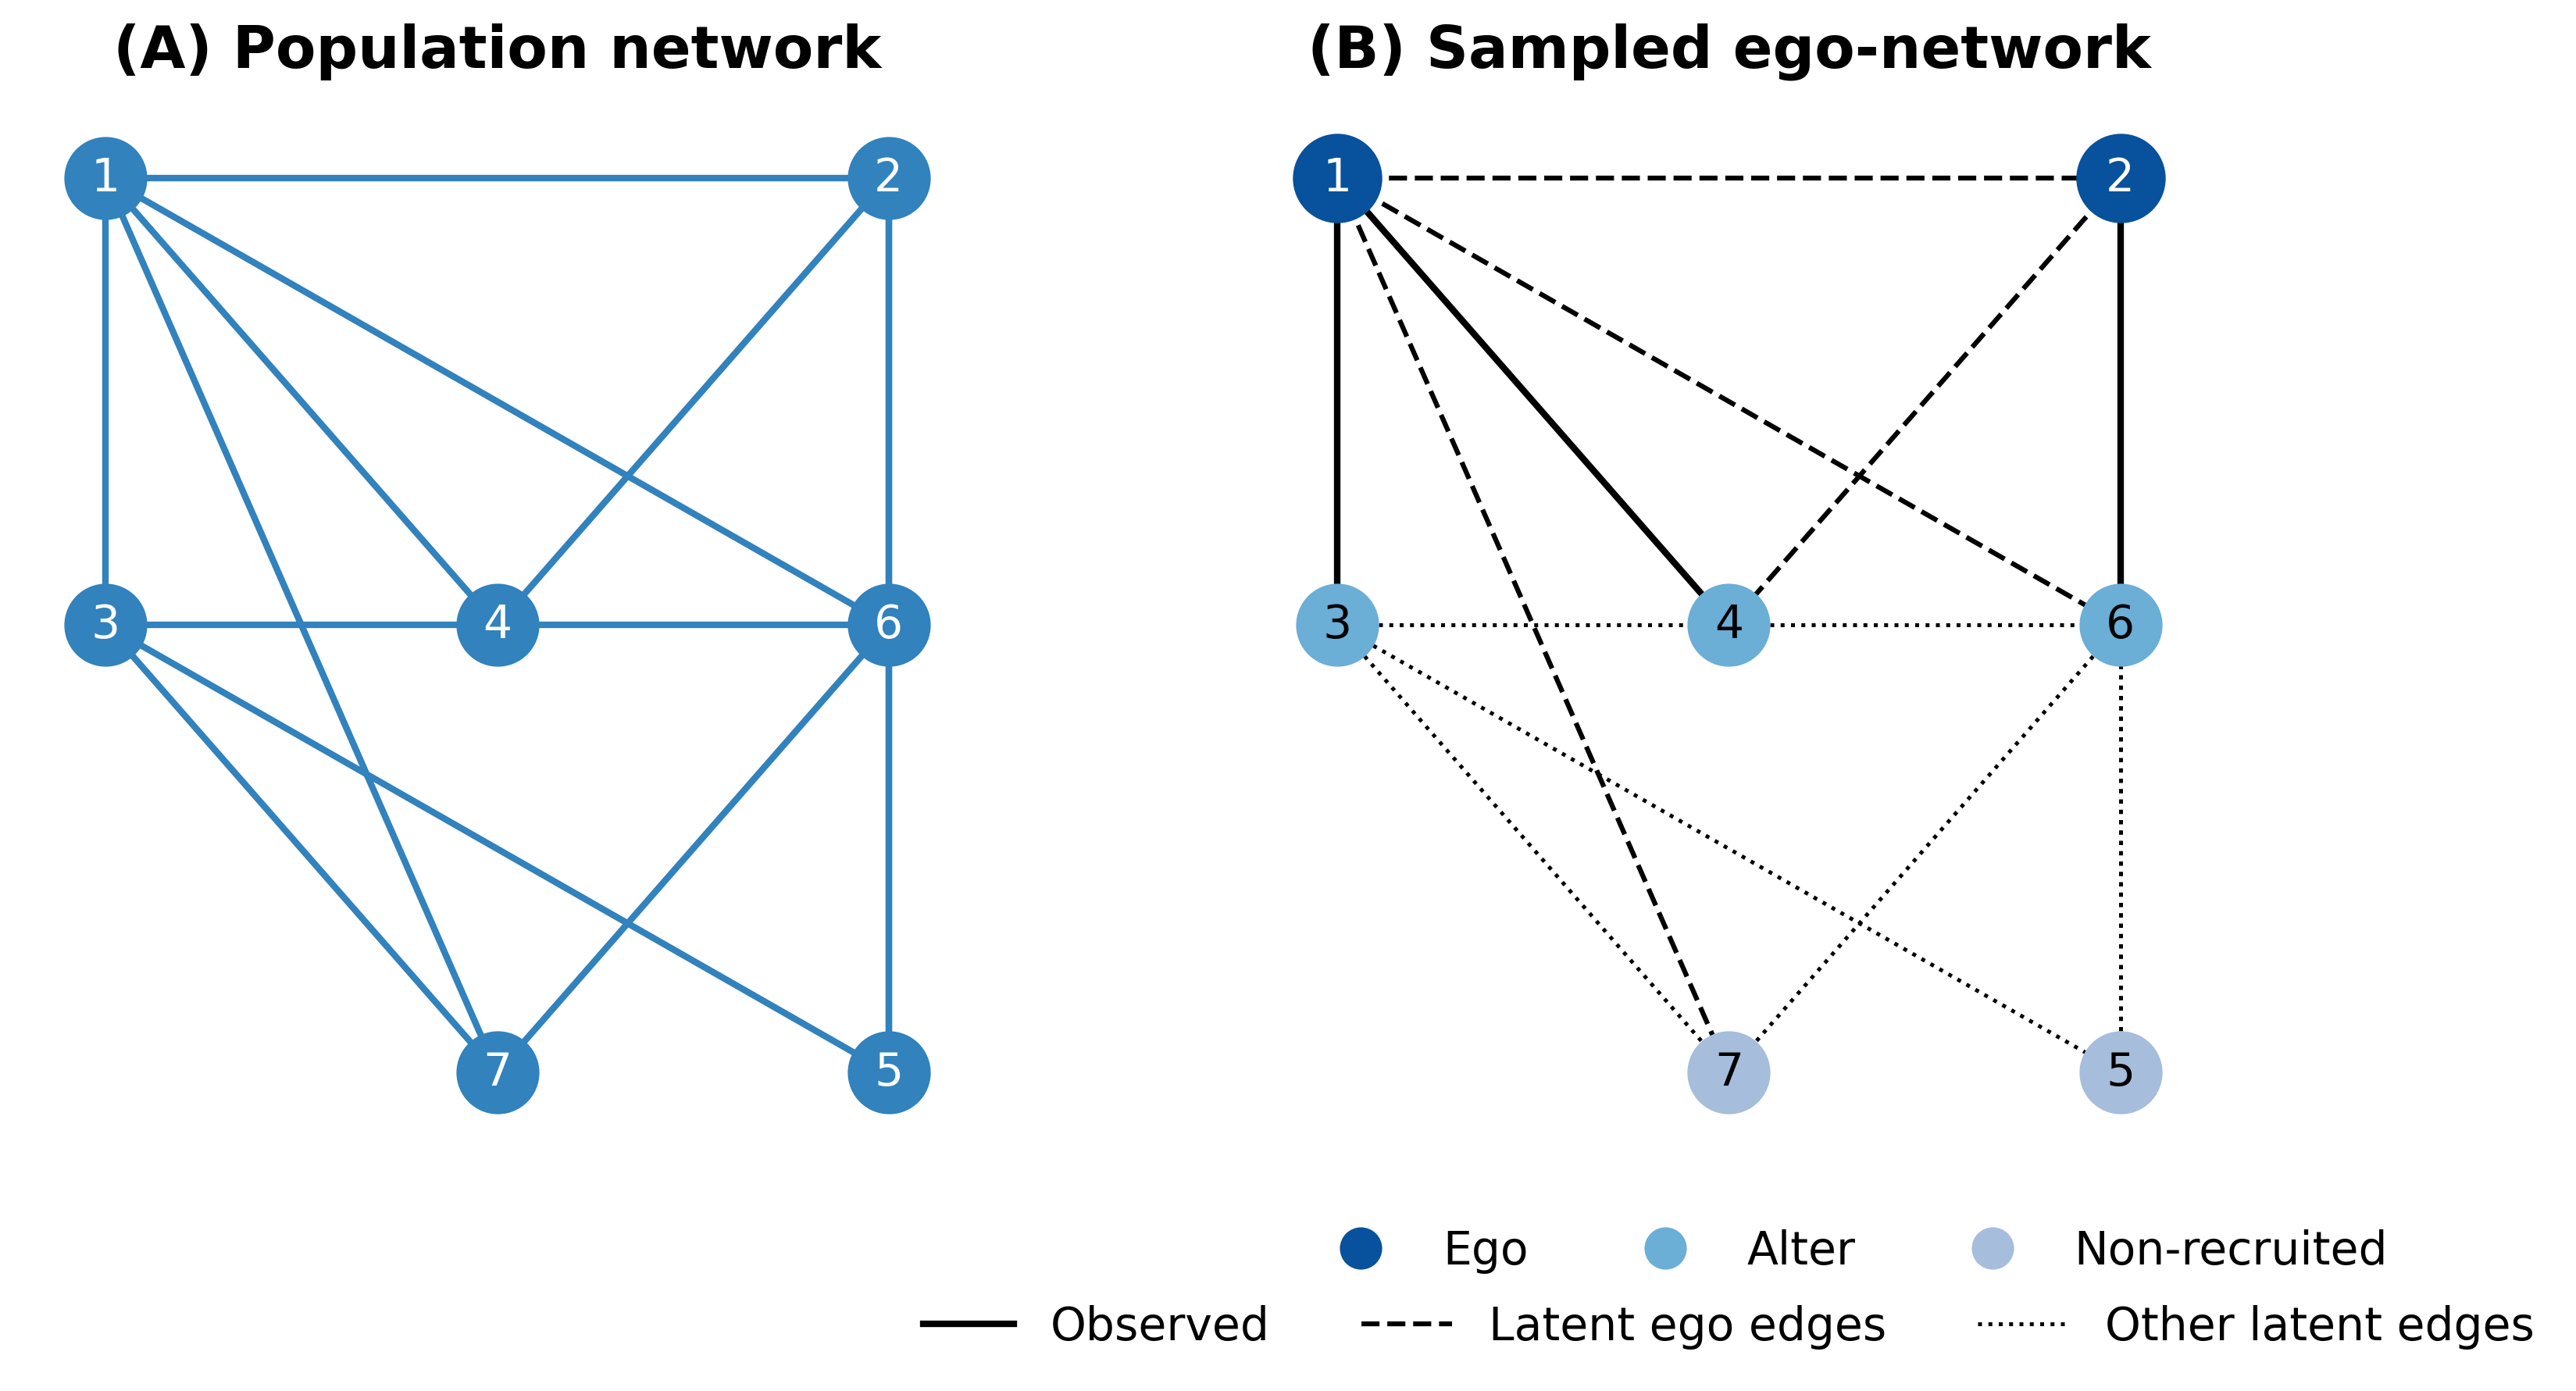
\includegraphics[width=0.7\linewidth]{figures/population_and_ego_network.png
    }
    \caption{Egocentric-network sampling. 
    Panel~(A) shows the full $N=7$ population network.
    Panel~(B) illustrates an egocentric-network sample: each ego (dark blue, $n_e=2$) reports only a subset of its true neighborhood as alters (medium blue, $n_a=3$).
    The observed network is composed of disjoint ego–networks stars (solid lines),
    while ego–ego and unreported ego–alter connections remain latent (dashed lines).
    All other edges are also unobserved (dotted lines).}
    \label{fig:egonetwork}
\end{figure}


\subsection{Experimental design, potential outcomes, and causal estimands}
\label{susec:doe_po_estimands}
In what follows, all assumptions, estimands, and estimators are conditioned on the recruited subsample. That is, we consider in-sample causal effects.
Let $\bZ$ be the binary treatment assignment vector, where $Z_i = 1$ if unit $i$ is treated, and $0$ otherwise.
Assume that treatments are randomly assigned to the recruited egos via Bernoulli randomization.
\begin{assumption}[Bernoulli experimental design]
\label{ass:bernoulli_design}
    Treatments are independently assigned only to recruited egos
    $\Pr(Z_i = 1 \mid \cR) = p_z 1\{i \in \cR_e\}$ where $p_z \in (0,1)$ is a known constant.
\end{assumption}
Denote the treatment space as $\mathcal{Z} = \left\{\bz \in \{0,1\}^N : \Pr(\bZ=\bz \mid \cR) > 0 \right\}$,
where treatments of non-recruited units are assumed to be equal to zero with probability one.
This experimental design,
in which treatments are randomized to egos following an egocentric-network sample,
is referred to as an \emph{egocentric-network randomized trial} (ENRT).

Let $Y_i(\bz)$ be the potential outcomes of each unit under treatment $\bz \in \mathcal{Z}$.
We take a randomization-based inference approach,
where the potential outcomes assumed to be fixed and the only source of randomness is due the treatment assignment. 
Let $\bZ_{-i}$ denote the treatment assignment of all units except $i$.
Assume that $\bZ_{-i}$ affects the potential outcomes of unit $i$ only
 through the values of the following exposure mapping \citep{Manski2013,aronow_estimating_2017,Forastiere2020}.
\begin{assumption}[Exposure mapping]
\label{ass:expos_map}
    Let $F(\bZ_{-i},\bA) =\mathbb{I}\left\{\sum_{j\neq i} Z_jA_{ij} > 0\right\}$. For any $\bz, \bz' \in \mathcal{Z}$, if $z_i = z'_i$ and $F(\bz_{-i},\bA) = F(\bz'_{-i},\bA)$, then $Y_i(\bz) = Y_i(\bz')$. 
\end{assumption}
Denote the exposures in the true population network by $F_i = F(\bZ_{-i}, \bA)$.
The exposures $F_i$ indicate whether at least one of the neighbors of unit $i$ is treated.
Assumption~\ref{ass:expos_map} states that the exposure mapping is correctly specified \citep{Saevje2023},
and imply that only treatments of neighbors affect the potential outcomes of unit $i$.
This binary exposure mapping specification is common in the ENRT literature \citep{Buchanan2018,Chao2023,Fang2023}.

By Assumption~\ref{ass:expos_map}, we can express the potential outcomes as
$Y_i(\bZ)=Y_i(Z_i,F_i)$.
Consequently, each unit has four effective potential outcomes,
$Y_i(z,f)$ for $z,f\in\{0,1\}$, indicating whether unit $i$ is treated and whether at least one of its neighbors is treated.
We assume that the observed outcomes $Y_i, \; i \in \cR$ are generated from one of the potential outcomes by:
\begin{assumption}[Consistency]
\label{ass:consis}
$Y_i = \sum_{z,f \in \{0,1\}}Y_i(z,f) \mathbb{I}\left\{Z_i=z, F_i=f\right\}$ for all $i \in \cR$.    
\end{assumption}
In addition, assume that we observe covariates $\bX_i$ for each recruited unit.

We consider two types of causal estimands, separate for egos and alters.
%  as common in the literature\footnote{There are interpretation issues with estimands such as $\EX\big[Y_i(1,0)-Y_i(0,1) \big]$, see \citet{Crawford2019}.}.
The first is the sample average indirect effects of treatment on the alters 
\begin{equation}
    \label{eq:indirect_effect}
    IE = 
    \frac{1}{n_a} 
    \sum_{i\in\cR_a}
    Y_i(0, 1) - Y_i(0,0).
\end{equation}
Eq.~\eqref{eq:indirect_effect} represents the average effect on alters of being exposed to a treated neighbor compared to not being exposed.
In Appendix~\ref{apdx_sec:proof}, we also consider the indirect effects on the relative risk scale, in the case of binary outcomes.

The second estimand is sample average direct effect of treatment on the egos direct effect of treatment on the egos
\begin{equation}
    \label{eq:directed_effect}
    DE = 
    \frac{1}{n_e}
    \sum_{i\in\cR_e}
    Y_i(1, 0) - Y_i(0,0).
\end{equation}
Eq.~\eqref{eq:directed_effect} represents the average effect on egos of being treated compared to not being treated when not exposed to any treated neighbors.

We explicitly separate the causal estimands for egos and alters.
This separation resolve interpretation issues of other estimands \citep{Crawford2019}.
Furthermore, by not conflating the two groups we avoid imposing additional assumptions and structure,
as the recruitment process (Section~\ref{subsec:recruitment}) may induce different selection mechanisms for egos and alters, 
leading to incomparable distributions of potential outcomes between the two groups.

\subsection{Estimation with the observed data}
Researchers have access only to the observed data composed of the treatment assignments $\bZ$,
the observed outcomes $Y_i, \; i \in \cR$, the observed network $\widetilde{\bA}$, and possibly
covariates $\bX_i$.
However, by Assumption~\ref{ass:consis}, the observed outcomes $Y_i$
are generated from the potential outcomes with exposures $F_i$ 
computed using the \emph{population network}.
The observed exposures are $\widetilde{F}_i = F(\bZ_{-i}, \widetilde{\bA})$,
which may differ from the true exposures $F_i$. 
That is, the observed network $\widetilde{\bA}$ might not capture all the relevant edges present in the population network $\bA$ 
due to the egocentric-network sampling process, resulting in \emph{misspecified network interference structure} \citep{Weinstein2023}.
We specifically care about missing ego-ego and additional alter-alter edges induced by the sampling process.

For example, in the context of Figure~\ref{fig:egonetwork},
if only ego 1 is treated, for alter 6 we observe exposure $\widetilde{F}_i=0$ since its ego (node 2) is not treated,
but its true exposure is $F_i=1$ due to its link to ego 1 in the population network. 
Similarly, for ego 2 we observe exposure $\widetilde{F}_i=0$ while $F_i=1$ in the population network
since it is connected to ego 1.

By the ENRT design, the observed exposures of egos are $\widetilde{F}_i =0$ for all $i \in \cR_e$,
while the observed exposures of alters can be either zero or one, depending on their ego's treatment status.
Specifically, by Assumption~\ref{ass:bernoulli_design}, alters are exposed to a treated ego
with probability $\Pr(\widetilde{F}_i=1 \mid i \in \cR_a) = p_z$.

Therefore, researchers can estimate causal effect only with the observed exposures.
The most common estimator in randomization-based inference settings is the Horvitz-Thompson (HT) estimator.
For the indirect effects \eqref{eq:indirect_effect}, its form is
\begin{equation}
    \label{eq:IE_naive_HT}
    \widehat{IE} = 
    \frac{1}{n_a}
    \sum_{i \in \cR_a}
    \left[
    \frac{
    \mathbb{I}\{\widetilde{F}_i=1\}Y_i}{p_z} 
    -
    \frac{
    \mathbb{I}\{\widetilde{F}_i=0\}Y_i}{1 - p_z} 
    \right],
\end{equation}
and for direct effects \eqref{eq:directed_effect},
\begin{equation}
    \label{eq:DE_naive_HT}
    \widehat{DE} = 
    \frac{1}{n_e}
    \sum_{i \in \cR_e}
    \left[
    \frac{
    \mathbb{I}\{Z_i=1\}Y_i}{p_z} 
    -
    \frac{
    \mathbb{I}\{Z_i=0\}Y_i}{1 - p_z} 
    \right].
\end{equation}
If some alter-ego or ego-ego edges are missing in the observed network $\widetilde{\bA}$ due to the egocentric-network sampling process,
then for some units the observed exposures $\widetilde{F}_i$ may not agree with the true exposures $F_i$ under all possible treatment assignments $\mathcal{Z}$.
In that case, both estimators \eqref{eq:IE_naive_HT} and \eqref{eq:DE_naive_HT} may not be design-unbiased.
\begin{proposition}
    \label{prop:bias_naive_ht}
    Under Assumptions~\ref{ass:bernoulli_design}, \ref{ass:expos_map}, \ref{ass:consis},
    \begin{equation*}
        \begin{aligned}
        \EX_{\bZ}\left[\widehat{IE} \right] 
        &=
        IE + 
        \frac{1}{n_a} 
    \sum_{i\in\cR_a}
    \frac{p_z -\pi_i^a}{1-p_z}
    \left[
    Y_i(0, 1) - Y_i(0,0)
    \right],
    \\
      \EX_{\bZ}\left[\widehat{DE} \right] 
        &=
        DE + 
        \frac{1}{n_e} 
    \sum_{i\in\cR_e}
    \pi_i^e
    \left[
    \left\{ Y_i(1, 1) - Y_i(0,1)\right\} 
    - \left\{ Y_i(1,0) - Y_i(0,0) \right\}
    \right],
        \end{aligned}
    \end{equation*}
    where $\pi_i^a = \Pr(F_i=1\mid i\in \cR_a)$ and $\pi_i^e = \Pr(F_i=1 \mid i \in \cR_e)$ are the probabilities that an alter and ego, respectively, are exposed to at least one treated neighbor in the population network $\bA$.
\end{proposition}
When an alter is connected only to its own ego, $\pi_i^a=p_z$, and \eqref{eq:IE_naive_HT} will be design-unbiased estimator of \eqref{eq:indirect_effect}.
Otherwise, whenever an alter is connected to more than one ego in the population network, $\pi_i^a > p_z$, and the indirect effect estimator \eqref{eq:IE_naive_HT} based on the observed exposures will be biased. 
The magnitude of the bias will depend on the number of egos each alter is connected to in the population network.
That is, the more egos an alter is connected to, the larger the gap between $\pi_i^a$ and $p_z$, and the larger the bias. 
In addition, the naive indirect estimator \eqref{eq:IE_naive_HT} is
attenuated towards the null of no indirect effect (Appendix~\ref{apdx_sec:proof}).

Furthermore, if an ego is not connected to any other ego in the population network, then $\pi_i^e=0$.
In that case, \eqref{eq:DE_naive_HT} will be a design-unbiased estimator of \eqref{eq:directed_effect}.
However, if an ego is connected to at least one other ego in the population network, then $\pi_i^e>0$,
and the direct effect estimator \eqref{eq:DE_naive_HT} based on the observed data will be biased.
Similarly to alters, the magnitude of the bias will depend on the number ego-ego edges to in the population network.
 
\section{Sensitivity analysis for contamination between ego-networks}
\label{sec:sa}

Proposition~\ref{prop:bias_naive_ht} shows that the HT estimators based on the observed data 
    are biased whenever there is contamination between the ego-networks.
We refer to contamination as the presence alter-ego and ego-ego edges in the population network $\bA$,
that are missing from the observed network $\widetilde{\bA}$ due to the egocentric-network sampling process.   
    
By the structure of the egocentric-network sampling and the
 exposure mapping specification (Assumption~\ref{ass:expos_map}),
alters with observed exposure $\widetilde{F}_i=1$ will be correctly classified. 
That is $\widetilde{F}_i=1$ implies $F_i=1$ with probability one for $i \in \cR_a$.
However, alters with $\widetilde{F}_i=0$ can have a true exposure of $F_i=1$ or $F_i=0$,
depending on the structure of the population network $\bA$.
That is, the observed outcomes $Y_i$ for alters with $\widetilde{F}_i=0$ can be generated from $Y_i(0,1)$ or $Y_i(0,0)$.

On the other hand, all egos have observed exposures of $\widetilde{F}_i=0$, 
as they are linked only to alters in their ego-network in the observed network $\widetilde{\bA}$.
Thus, the observed outcomes of egos that are assigned to
 treatment $Z_i=z$ can be generated from $Y_i(z,1)$ or $Y_i(z,0)$,
 implying that observed outcomes of egos are possibly linked to four different potential outcomes,
  compared to only two among the alters.

We develop a sensitivity framework that enables researchers to assess the impact of
 possible contamination between ego-networks on their causal estimates.
The framework provides bias-corrected estimators of the indirect and direct effects 
that account for possible exposure misspecification due to the egocentric-network recruitment process. 

 The bias-corrected indirect and direct effect estimators are a function of the
exposure probabilities under the true population network $\pi_i^a$ and $\pi_i^e$, respectively.
The structure of the egocentric-network sampling design and our setup 
allow us to decompose $\pi_i^a$ and $\pi_i^e$ into basic
 components that are straightforward to compute given specification
  of the \emph{expected number} or the \emph{probability} of alter-ego and ego-ego edges.
 The latter will form the basis of our sensitivity parameters, 
 enabling seamless integration of covariates and prior knowledge into the sensitivity analysis.
 We provide numerous examples and practical guidelines on how to specify these parameters in Section~\ref{subsec:rho_param}.
 
 For the direct effects, we require an additional sensitivity parameter 
    to account for the additional complexity of four possible potential outcomes generating the observed ones.
This parameter is related to the magnitude of the treatment and exposure interaction effect on the egos,
and its specifics are discussed in Section~\ref{subsec:de}.


\subsection{Indirect effects}
\label{subsec:ie}
Define the bias-corrected indirect effect estimator as a function of the observed data and $\pi_i^a$
\begin{equation}
    \label{eq:IE_corrected}
    \widehat{IE}_{adj} = 
    \frac{1}{n_a}
    \sum_{i \in \cR_a}
    \frac{1-p_z}{1-\pi_i^a}
    \left[
    \frac{
    \mathbb{I}\{\widetilde{F}_i=1\}Y_i}{p_z} 
    -
    \frac{
    \mathbb{I}\{\widetilde{F}_i=0\}Y_i}{1 - p_z} 
    \right],
\end{equation}
Given $\pi_i^a$, \eqref{eq:IE_corrected} is a design-unbiased estimator of \eqref{eq:indirect_effect}
\begin{proposition}
\label{prop:ie_sa}
  Under Assumptions~\ref{ass:bernoulli_design}, \ref{ass:expos_map}, \ref{ass:consis}, we have
  $\EX_{\bZ}\left[\widehat{IE}_{adj} \right] = IE$.
\end{proposition}

By the ENRT design and Assumptions~\ref{ass:expos_map}, $\pi_i^a \geq p_z$,
 with equality if and only if there are no additional latent alter-ego edges.
 Consequently, if each alter has the same exposure probabilities $\pi^a_i = \pi^a$,
 then $\widehat{IE}_{adj} = \frac{1-p_z}{1-\pi^a} \widetilde{IE}$.
 Therefore, $\text{sign}\left(\widehat{IE}_{adj}\right) = \text{sign}\left(\widetilde{IE}\right)$, 
 and $\widehat{IE}_{adj} \geq \widehat{IE}$ if $\widehat{IE} >0$ and vice versa otherwise.


The bias-corrected estimator \eqref{eq:IE_corrected} can be modified to include an outcome model.
 Let $m^a_i(f) = \EX \left[Y_i \mid \widetilde{F}_i=f, \bX_i, i \in \cR_a \right]$
be the conditional expectation among alters with observed exposure $\widetilde{F}_i = f$ and covariates $\bX_i$.
The augmented bias-corrected estimator is
\begin{equation}
    \label{eq:IE_corrected_aipw}
    \begin{aligned}
    \widehat{IE}_{adj}^{aug} 
    &= 
    \frac{1}{n_a}
    \sum_{i \in \cR_a}
    \frac{1-p_z}{1-\pi_i^a}
    \Bigg[
    \frac{
    \mathbb{I}\{
    \widetilde{F}_i=1\}\left(Y_i - m^a_i(1) \right)}{p_z} -
    \\ &\qquad \qquad \qquad
    \frac{
    \mathbb{I}\{\widetilde{F}_i=0\}\left(Y_i - m^a_i(0) \right)}{1 - p_z} 
    + \left\{m^a_i(1) - m^a_i(0) \right\}
    \Bigg].
    \end{aligned}
\end{equation}
Given that $m_i^a(f)$ are estimated in a way that ensure their independence from the treatment assignment $\bZ$,
e.g., via cross-fitting \citep{Chernozhukov2018},
then \eqref{eq:IE_corrected_aipw} is also a design-unbiased estimator of \eqref{eq:indirect_effect}, but can have lower variance.

Given $\pi_i^a$, the variance of the bias-corrected estimators \eqref{eq:IE_corrected} and \eqref{eq:IE_corrected_aipw}
can be estimated using standard techniques for HT estimators under Bernoulli designs or 
thorough a nonparameteric bootstrap that resamples ego-networks (see Appendix~\ref{apdx_sec:proof} for details).

\subsection{Direct effects}
\label{subsec:de}

As the observed outcomes of egos are possibly generated from four different potential outcomes,
 compared to only two for the alters, bias correction for the direct effect estimator requires an additional structural assumption. 
 Specifically, we require that the unit-level direct effects among exposed ($F_i=1$) and non-exposed ($F_i=0$) egos are proportional
\begin{assumption}
    \label{ass:egos_kappa}
    There exists a constant $\kappa$ such that 
    $Y_i(1,1) - Y_i(0,1) = \kappa \left\{Y_i(1,0) - Y_i(0,0)\right\}$ for all egos $i \in \cR_e$.
\end{assumption}
The interpretation of the additional sensitivity parameter $\kappa$ in
 Assumption~\ref{ass:egos_kappa} is related to the interaction term between treatment and exposure in the potential outcome model of the egos.
  Consider the saturated potential outcomes model
\begin{equation*}
    Y_i(z,f) = \beta_{0i} + \beta_{1i}z + \beta_{2i}f + \beta_{3i}zf,
\end{equation*}
then Assumption~\ref{ass:egos_kappa} is equivalent to $\beta_{3i} = (\kappa-1)\beta_{1i}$. 
That is, the interaction term $\beta_{3i}$ is proportional to the direct effect term $\beta_{1i}$ for all egos.
Reasoning about the range of plausible $\kappa$ values depends on the mechanism under study. 
For example, in vaccine efficacy studies, if treatment represents vaccines, 
it is reasonable to assume that direct effects among egos with only non-vaccinated neighbors 
will be larger than those among egos exposed to vaccinated units, and therefore $\kappa < 1$.
On the other hand, in the HPTN-037 study \citep{Latkin2009}, 
    which we analyze in Section~\ref{sec:data},
    treatment represent a behavioral intervention.
    Such intervention is likely to have monotonic effects, namely,
    the direct effect is likely to be larger for egos with exposed to treated neighbors, leading to $\kappa > 1$.
    
Define the the bias-corrected direct effect estimator as a function of the observed data, $\pi_i^e$, and $\kappa$
\begin{equation}
    \label{eq:DE_corrected}
    \widehat{DE}_{adj} =
    \frac{1}{n_e}
    \sum_{i \in \cR_e}
    \frac{1}{1 + \pi_i^e(\kappa-1)}
    \left[
    \frac{
    \mathbb{I}\{Z_i=1\}Y_i}{p_z} 
    -
    \frac{
    \mathbb{I}\{Z_i=0\}Y_i}{1 - p_z} 
    \right]
\end{equation}
\bwnote{TODO: continue here.}

Given $\pi_i^e$ and $\kappa$, \eqref{eq:DE_corrected} is a design-unbiased estimator of \eqref{eq:directed_effect}
\begin{proposition}
\label{prop:de_sa}
    Under Assumptions~\ref{ass:bernoulli_design}, \ref{ass:expos_map}, \ref{ass:consis}, \ref{ass:egos_kappa}, we have
     $\EX_{\bZ}\left[\widehat{DE}_{adj} \right] = DE$.
\end{proposition}

If $\pi_i^e=0$ or $\kappa=1$, the bias-corrected estimator will reduce to the naive HT estimator, and both will be unbiased.

\bwnote{Write about the grid of $\kappa$ values and what it means about attenuation or not towards the null.
We do require that $\kappa \neq 1 - \frac{1}{\pi_i^e}$ for all $i\in \cR_e$ for the estimator to be well defined.}


\bwnote{Refine the paragraph.} Extension also to augmented bias-corrected estimator as in \eqref{eq:IE_corrected_aipw}. Here $m^e_i(z) = \EX \left[Y_i \mid Z_i =z, \bX_i, i \in \cR_e \right]$.
\begin{equation}
    \label{eq:DE_corrected_aipw}
    \widehat{DE}_{adj}^{aug} = 
    \frac{1}{n_e}
    \sum_{i \in \cR_e}
    \frac{1}{1 + \pi_i^e(\kappa-1)}
    \left[
    \frac{
    \mathbb{I}\{
    Z_i=1\}\left(Y_i - m^e_i(1) \right)}{p_z} 
    -
    \frac{
    \mathbb{I}\{Z_i=0\}\left(Y_i - m^e_i(0) \right)}{1 - p_z} 
    + \left\{m^e_i(1) - m^e_i(0) \right\}
    \right],
\end{equation}

\subsection{Specification of the sensitivity parameter}
\label{subsec:rho_param}
Propositions~\ref {prop:ie_sa}-\ref{prop:de_2param_sa} establish the relationships between indirect \eqref{eq:indirect_effect} and direct \eqref{eq:directed_effect} estimands, the naive estimators \eqref{eq:indirect_effect_estimator}-\eqref{eq:directed_effect_estimator}, and the marginal probabilities of exposures in the population network $\pi^e_i$ and $\pi^a_i$.
In the case of indirect effects among alters, we have point identification given $\pi^a_i$. For direct effects among egos, we develop a one-parameter sensitivity analysis on bounds of the direct effects and a two-parameter sensitivity analysis for point identification. Both depend on $\pi^e_i$. Let $\cR_e^{i} =\cR_e \setminus \{i\}$ be the set of egos excluding $i$.

Since treatments are randomly assigned only to recruited units (Assumption~\ref{ass:bernoulli_design}) and exposures $F_i$ indicates whether a unit is exposed to at least one treated neighbor (Assumption~\ref{ass:expos_map}), the probabilities $\pi^a_i$ and $\pi^e_i$ depend only on alter-ego or ego-ego edges that are missing due to the egocentric recruitment process (dashed edges in Figure~\ref{fig:egonetwork}). 
Specifically, the ego-ego edges $\left\{A_{ij}: i,j \in \cR_e\right\}$ and alter-ego edges between ego-networks $\left\{A_{ij} : i \in \cR_a, j \in \cR_e^{e(i)} \right\}$ are latent.
The proposed sensitivity analysis will be expressed in terms of probabilities on these missing edges\footnote{This sensitivity analysis will be a weaker assumption than a full prior network model. We only require the specifications of edge probabilities for a subset of missing edges.}. 
Define the edge-level probabilities by
\begin{equation}
    \label{eq:sbm}
    \begin{aligned}
    &\Pr\left(A_{ij}=1 \mid i,j \in\cR_e\right) = \rho^e_{ij},
    \\ 
    &\Pr\left(A_{ij}=1 \mid i \in \cR_a, j \in \cR_e^{e(i)} \right) = \rho^a_{ij},
    \end{aligned}
\end{equation}
for $\rho^e_{ij}, \rho^a_{ij} \in [0,1]$.
Using \eqref{eq:sbm}, we can derive expressions for $\pi^e_i$ and $\pi^a_i$.
Starting with $\pi^e_i$,
By the law of total probability,
\begin{equation*}
    % \Pr(Z_jA_{ij} = 0 \mid i,j \in \cR_e) 
    % =
    % 1 - \Pr(Z_jA_{ij} = 1 \mid i,j \in \cR_e)
    \Pr\left(Z_jA_{ij} = 1 \mid i,j \in \cR_e\right)
    =
    p_z\rho^e_{ij}.
    % 1 - p_z\rho^e_{ij}.
\end{equation*}
The event $F_i=0$ is equivalent to $Z_jA_{ij} = 0$ for all $j \in \cR_e^i$. Assuming (conditional) edge independence yields,
\begin{equation}
    \label{eq:pi_ego}
    \pi^e_i = 1 - \prod_{j \in  \cR_e^i}
    \big(1 - p_z \rho^e_{ij}\big).
\end{equation}
For alters $i\in\cR_a$, $F_i=1$ if its ego $e(i)$ or at least one of the other recruited egos connected to $i$ in the population network $\bA$ is treated. Therefore, we obtain (Appendix~\ref{apdx_sec:proof}),
\begin{equation}
    \label{eq:pi_a}
    \pi^a_i = p_z + 
    (1-p_z)
    \left[1- \prod_{j \in  \cR_e^{e(i)}}
    \big(1 - p_z \rho^a_{ij}\big)\right]
    = 
    1 - (1-p_z)\prod_{j \in  \cR_e^{e(i)}}
    \big(1 - p_z \rho^a_{ij}\big),
\end{equation}
and $\pi^a_i \geq p_z$ as stated in Section~\ref{subsec:ie}.

Eqs.~\eqref{eq:pi_ego}-\eqref{eq:pi_a} imply that the sensitivity analyses for indirect and direct effects demand specification of $\rho^e_{ij}$ and $\rho^a_{ij}$ by the researchers. We now consider some prominent examples.  

\begin{exmp}[Homogeneous probabilities]
    \label{exmp:pi_homo}
    The probabilities in \eqref{eq:sbm} are the same for all units:
    $\rho^e_{ij}=\rho^e$ and $\rho^a_{ij}=\rho^a$. The product in \eqref{eq:pi_ego} is reduced to,
    \begin{equation*}
        \prod_{j \in \cR_e^i}
    \big(1 - p_z \rho^e_{ij}\big) = (1-p_z\rho^e)^{n_e-1},
    \end{equation*}
    and similarly to \eqref{eq:pi_a} with $\rho^a$.
\end{exmp}

\begin{exmp}[Number of missing edges]
    \label{exmp:pi_number}
    A special case of Example~\ref{exmp:pi_homo} occurs when the researchers specify the total \emph{expected} number of missing edges, separately for the ego-ego and alter-ego edges. 
    If $m^e \in \left\{1,\ldots, \binom{n_e}{2}\right\}$ is the expected number of ego-ego edges that are believed to be missing, then set
    \begin{equation*}
        \rho^e_{ij} = \rho^e(m^e) = \frac{m^e}{\binom{n_e}{2}}.
    \end{equation*}
    There are $n_a(n_e-1)$ possible missing alter-ego edges between alters and egos from different ego-networks. If $m^a$ such edges are expected to be missing, set 
    \begin{equation*}
        \rho^a_{ij} = \rho^a(m^a) = \frac{m^a}{n_a(n_e-1)}.
    \end{equation*} 
\end{exmp}

\begin{exmp}[Heterogeneous probabilities]
    \label{exmp:pi_hetero}
    Examples~\ref{exmp:pi_homo}-\ref{exmp:pi_number} can be extended to incorporate unit-level characteristics through covariates $\bX_i$. 
    A well-known result in network science is homophily, which states that units with similar characteristics are more likely to have social interactions.
    For scalar $\gamma^e \geq 0$ we can define
    similarity weights $w_{ij}^e = \exp \left(-\gamma^e d(\bX_i, \bX_j)\right)$ 
     for distance function $d(\cdot, \cdot)$, e.g., the Euclidean distance $d(\bx_i,\bx_j)=\lVert\bx_i - \bx_j\rVert$ or the cosine distance $d(\bx_i,\bx_j)=1 - \frac{\bx_i^T\bx_j}{\lVert \bx_i \rVert \lVert \bx_j \rVert}$. 
    Alternatively, it is possible to use the inner product, $w_{ij}^e = \exp \left(\gamma^e \bX_i^T\bX_j\right)$.
    And then set ego-ego edge probabilities to
    \begin{equation*}
     \rho^e_{ij}=\frac{w_{ij}^e}{\sum_{j \in \cR_e^i}w_{ij}^e}.
    \end{equation*}
    In both cases, $\gamma^e$ controls the influence of covariate similarity: $\gamma^e \to 0$ yields uniform probabilities $\rho^e_{ij} \to\frac{1}{n_e-1}$, while larger $\gamma^e$ concentrates mass on more closer or similar nodes. Analogous definitions apply for alter-ego edges with weights $w_{ij}^a$, probabilities $\rho^a_{ij}$, and a sensitivity parameter $\gamma^a \geq 0$.   
\end{exmp}

\begin{exmp}[Heterogeneous number of missing edges]
\label{exmp:pi_hetero_number}
    Examples~\ref{exmp:pi_number}–\ref{exmp:pi_hetero} can be combined to allow pair-specific heterogeneous probabilities while fixing only the total expected number of missing edges.
    Let $w_{ij}^e$ and $w_{ij}^a$ be the weights defined in Example~\ref{exmp:pi_hetero} with $\gamma^e=\gamma^a=1$.
    Define the total sum of weights among ego-ego and alter-ego pairs with missing edges,
    \begin{equation*}
     W^e=\sum_{i<j\in \cR_e}w_{ij}^e, \qquad W^a = \sum_{i\in \cR_a}\sum_{j \in \cR_e^{e(i)}} w_{ij}^a.   
    \end{equation*}
    Similarly to Example~\ref{exmp:pi_number}, specify the expected numbers $m^e$ and $m^a$ of missing ego-ego and alter-ego edges, and set
    \begin{equation*}
        \rho^e_{ij}=\frac{m^e}{W^e}\,w^e_{ij},
        \qquad
        \rho^a_{ij}=\frac{m^a}{W^a}\,w^a_{ij}.
    \end{equation*}
    If $m^e \geq W^e$ or $m^a \geq W^a$, the probabilities must be capped to ensure that $\rho_{ij}\leq 1$. We describe a simple procedure for this scenario in Appendix~\ref{apdx_sec:proof}. Setting all weights to one recovers Example~\ref{exmp:pi_number}.
\end{exmp}

\textbf{TODO: this capping I described doesn't ensure that each unit attains the bounded degree mentioned. That follows from the symmetry of edges in undirected networks. Need to either modify this solution (e.g., via greedy matching or top-d pruning that will define the feasible set of edges) or just remove it.}

Examples~\ref{exmp:pi_homo}-\ref{exmp:pi_hetero} implicitly allow every latent ego-ego and alter-ego edge to exist.
Suppose instead that each ego can form at most $d^e_{max}$ latent ego-ego ties and each node (ego or alter) at most $d^a_{max}$ latent alter-ego ties. 
The probabilities in the examples can be modified as follows.
\begin{enumerate}
    \item \textbf{Example~\ref{exmp:pi_homo}.} Replace the exponent $n_e-1$ with $\min\left(n_e-1, d^e_{max}\right)$. Make the same substitution for the alter-ego exponent with $d^a_{max}$.
    \item \textbf{Example~\ref{exmp:pi_number}.}
    Now there are at most $M^e_{max}=\min \left(\binom{n_e}{2}, \frac{n_e d^e_{max}}{2}\right)$ latent ego-ego edges available. Set $\rho^e(m^e) = \frac{m^e}{M^e_{max}}$ for $m^e \in \{1,\ldots, M^e_{max}\}$. 
    For alter-ego edges, the total bipartite edges is $M^a_{max} = \min \left(n_a(n_e-1),n_ed^a_{max},n_ad^a_{max}\right)$, so we define $\rho^a(m^a) = \frac{m^a}{M^a_{max}}$.
    \item \textbf{Example~\ref{exmp:pi_hetero}.} Compute the weights $w_{ij}^e$, keep the $d^e_{max}$ largest weights for each ego (receptively, $d^a_{max}$ for each alter-ego with $\gamma^a$), set the rest to zero, and then renormalize the retained weights so they sum to one.
\item \textbf{Example~\ref{exmp:pi_hetero_number}.}
Start from the weights of Example~\ref{exmp:pi_hetero}. 
For ego–ego pairs, for each ego keep its $d^e_{\max}$ largest weights and set the rest to zero; retain an edge $i\!<\!j$ only if it is in both endpoints’ top-$d^e_{\max}$ lists (mutual top-$d$). 
For alter–ego pairs, apply the same pruning with $d^a_{\max}$ on \emph{both} sides (mutual top-$d^a_{\max}$). 
\end{enumerate}
Let $\widetilde{d}_i$ be the observed degree in the ego-network $\widetilde{\bA}$. Since each alter is connected only to its own ego, $\widetilde{d}_i=1$ for $i \in \cR_a$. After adding the possible latent edges, the maximal degrees are
\begin{equation*}
    d_{max}(i) = 
    \begin{cases}
        \widetilde{d}_i + d^e_{max} + d^a_{max},
        & i \in \cR_e, \\
        1 + d^a_{max}, & 
        i \in \cR_a.
    \end{cases}
\end{equation*}
These caps ensure that the modified probabilities remain valid inputs to \eqref{eq:pi_ego}-\eqref{eq:pi_a}. 

\paragraph{Degree-feasible support via greedy pruning.}
For ego–ego pairs, sort all candidate pairs $(i,j)$ by weight $w^e_{ij}$ (in the homogeneous case, use any fixed symmetric tie-break). 
Scan in that order and add $(i,j)$ to the support $S_e$ if both endpoints currently have degree $< d^e_{\max}$; otherwise skip. 
Stop when no more pairs can be added or when $|S_e|=M^e_{\max}=n_e d^e_{\max}/2$.
For alter–ego pairs, apply the same rule on the bipartite graph (respecting the exclusion of $j^\star(i)$ and the cap $d^a_{\max}$ on \emph{both} sides) to obtain $S_a$.
All sums/products “over available pairs” in Examples~\ref{exmp:pi_homo}–\ref{exmp:pi_hetero_number} are then taken over $S_e$ or $S_a$ (with $W^e,W^a$ replaced by the corresponding totals over these supports). 
Selecting the top $M_{\max}$ pairs \emph{without} the degree check enforces only a global bound and can violate node caps; the greedy rule enforces both.
(If any resulting $\rho_{ij}>1$, apply the global capping procedure in Appendix~\ref{apdx_sec:proof}.)



\subsection{Practical considerations}
\label{subsec:practice}

The proposed sensitivity analyses are flexible and are compatible with any statistical model for the conditional mean of the outcomes with the observed exposures $\widetilde{F}_i$, and possibly covariates $\widetilde{\bX}_i$. To avoid imposing additional structural assumptions on the differences of potential outcomes of egos and alters, we recommend estimating two conditional outcome models, separately for egos and alters.  

Given the sensitivity parameters $\rho^a_{ij}, \rho^e_{ij}$, and possibly $\kappa$, the researchers can run the sensitivity analyses and obtain estimates or bounds for the estimands under study. Accounting for sampling uncertainty in both the estimated outcome model on the observed exposures and the exposure probabilities is possible through a non-parametric bootstrap. Due to possible dependence between units, we recommend to resample ego-networks rather than individual units. 

Given a grid of sensitivity parameters, the full procedure can be performed as follows. \bwnote{Updated the high-level structure that includes the outcomes models $m^a, m^e$ as well.}
\begin{enumerate}[label = (\roman*)]
    \item \label{sa:step1} Estimate the outcome models 
    $m^a_i(f), m^e_i(z)$. Use cross-fitting via $k$-fold split (deafult can be two-fold split, namely, split data into two folds (e.g., split into two folds of ego-networks), estimate outcome model in one fold and predict $m^e_i, m^a_i$ on the data from the second one, and vice versa). If not using the augmented estimators, we can set $m^e_i = m^a_i = 0$.
    \item \label{sa:step2} For each parameter in the grid of sensitivity parameters, obtain bias-corrected estimates of IE \eqref{eq:IE_corrected}-\eqref{eq:IE_corrected_aipw} and DE \eqref{eq:DE_corrected}-\eqref{eq:DE_corrected_aipw}.
    \item \label{sa:step3} Estimate variance of both IE and DE bias-corrected estimator as a function of the SA parameters... we have a closed-form expression here.
    \item \label{sa:step4} Compute confidence intervals for the bias-corrected estimates using normal approximation.
\end{enumerate}

The interpretation of the sensitivity analyses results can follow other traditional approaches. That is, by observing what parameter values change the sign of the naive estimates. It will enable researchers to reason about the maximal level of contamination required to change the conclusion of the study.

\textbf{TODO: this 'deterministic' sensitivity analysis approach can be modified to Probabilistic bias analysis (PBA) \citep{Greenland2005, Lash2014} by taking a prior distribution on the sensitivity parameter $p(\rho^e)$, and instead of computing bias-corrected estimated for each sensitivity parameter value, replace Step~\ref{sa:step2} with multiple samples $\rho^e\sim p(\rho^e)$ and obtain bias-corrected estimates as the average of the bias-corrected estimates for each $\rho^e$ sample.}

\textbf{TODO: As we have a variance estimator expression given any value of the SA parameters, we can use normal approximation to obtain PBA interval accounting for both design uncertainty (over $\bZ$ distribution) and bias uncertainty (from prior of SA params).}

\section{Simulation study}
\label{sec:sim}
DGP that mimics the settings of HPTN 037. The average number of edges was $2$. In it, each ego recruited at least one network member (drug injection or sexual partner). We can have the following settings

\begin{enumerate}
    \item Population network $\bA$ from SBM with $\{250,500,1000\}$ clusters. Each contain $[2,6]$ members (random uniform or truncated Poisson for cluster size). Between clusters probs $p_b \in \{0.01,0.05\}$ that will play the role of $\rho^a,\rho^e$. The between-cluster probs $p_b$ will generate the contamination. Can take either homogeneous or heterogeneous probabilities. 
    \item Each cluster in the SBM can represent one ego-network, so we can randomly sample one unit from each cluster to be an ego, and sample $\min(d_i,2)$ other units from its cluster as alters. Then, we randomize treatments to egos $p_z=0.5$ (as in HPTN 037).
    \item Generate potential outcomes from logistic model $\Pr(Y_i(z,f))=g^{-1}(\beta_0 + \beta_1 z +\beta_2f + \beta_3 zf)$.
    To satisfy Assumption~\ref{ass:spillovers_ego_alter}, $\beta_0, \beta_2$ should be the same for egos and alters. Also, $\kappa$ in Assumption~\ref{ass:egos_kappa} is approximate $\exp(\beta_3)$ as described in Example~\ref{exmp:logistic_po}.
    \item 
    Run the sensitivity analyses using Propositions~\ref{prop:ie_sa}-\ref{prop:de_2param_sa}, where $\rho^e_{ij}=\rho^a_{ij}=0$ returns the naive estimates \eqref{eq:indirect_effect_estimator} and \eqref{eq:directed_effect_estimator}.
    \item In Step~4, can do SA with both homogeneous (Examples~\ref{exmp:pi_homo}-\ref{exmp:pi_number}) and heterogeneous (Example~\ref{exmp:pi_hetero}) sensitivity edge probabilities. One of them will always be misspecified (depending on the network model used).
    \item Can modify the outcome model by including a random effect of ego-network to create dependence within clusters.
    \item Report results separately for indirect and direct effects. For direct effects, also separate the bounds from the bias correction with the addition of $\kappa$.
\end{enumerate}
Think about how to report the results.

{\renewcommand{\arraystretch}{0.8} % Shrink row height to 80% (adjust 0.8 as needed)
\begin{table}[H]

\caption{IE Results - Heterogeneous Exposure - Augmented}
\centering
\begin{tabular}[t]{lccccc}
\toprule
Scenario & spec & Variance & bias & coverage & ese\_ase\\
\midrule
 &  & Analytic & 0.016 & 0.978 & 0.774\\
\cmidrule{3-6}
 & \multirow{-2}{*}{\centering\arraybackslash Heterogeneous} & Bootstrap & 0.016 & 0.978 & 0.770\\
\cmidrule{2-6}
 &  & Analytic & 0.015 & 0.979 & 0.771\\
\cmidrule{3-6}
 & \multirow{-2}{*}{\centering\arraybackslash Homogeneous} & Bootstrap & 0.015 & 0.981 & 0.770\\
\cmidrule{2-6}
 &  & Analytic & -0.029 & 0.951 & 0.772\\
\cmidrule{3-6}
\multirow{-6}{*}[1\dimexpr\aboverulesep+\belowrulesep+\cmidrulewidth]{\raggedright\arraybackslash $m_a=100, IE=0.358$} & \multirow{-2}{*}{\centering\arraybackslash Naive} & Bootstrap & -0.029 & 0.951 & 0.773\\
\cmidrule{1-6}
 &  & Analytic & 0.006 & 0.977 & 0.839\\
\cmidrule{3-6}
 & \multirow{-2}{*}{\centering\arraybackslash Heterogeneous} & Bootstrap & 0.006 & 0.977 & 0.841\\
\cmidrule{2-6}
 &  & Analytic & 0.008 & 0.977 & 0.828\\
\cmidrule{3-6}
 & \multirow{-2}{*}{\centering\arraybackslash Homogeneous} & Bootstrap & 0.008 & 0.978 & 0.829\\
\cmidrule{2-6}
 &  & Analytic & -0.068 & 0.678 & 0.829\\
\cmidrule{3-6}
\multirow{-6}{*}[1\dimexpr\aboverulesep+\belowrulesep+\cmidrulewidth]{\raggedright\arraybackslash $m_a=200, IE=0.335$} & \multirow{-2}{*}{\centering\arraybackslash Naive} & Bootstrap & -0.068 & 0.678 & 0.829\\
\cmidrule{1-6}
 &  & Analytic & -0.004 & 0.972 & 0.906\\
\cmidrule{3-6}
 & \multirow{-2}{*}{\centering\arraybackslash Heterogeneous} & Bootstrap & -0.004 & 0.972 & 0.904\\
\cmidrule{2-6}
 &  & Analytic & 0.003 & 0.971 & 0.902\\
\cmidrule{3-6}
 & \multirow{-2}{*}{\centering\arraybackslash Homogeneous} & Bootstrap & 0.003 & 0.970 & 0.904\\
\cmidrule{2-6}
 &  & Analytic & -0.097 & 0.453 & 0.904\\
\cmidrule{3-6}
\multirow{-6}{*}[1\dimexpr\aboverulesep+\belowrulesep+\cmidrulewidth]{\raggedright\arraybackslash $m_a=300, IE=0.318$} & \multirow{-2}{*}{\centering\arraybackslash Naive} & Bootstrap & -0.098 & 0.451 & 0.902\\
\bottomrule
\end{tabular}
\end{table}
}


{\renewcommand{\arraystretch}{0.8} % Shrink row height to 80% (adjust 0.8 as needed)
\begin{table}[H]

\caption{DE Results - Heterogeneous Exposure - Augmented}
\centering
\begin{tabular}[t]{lccccc}
\toprule
Scenario & spec & Variance & bias & coverage & ese\_ase\\
\midrule
 &  & Analytic & 0.013 & 0.966 & 0.860\\
\cmidrule{3-6}
 & \multirow{-2}{*}{\centering\arraybackslash Heterogeneous} & Bootstrap & 0.013 & 0.964 & 0.864\\
\cmidrule{2-6}
 &  & Analytic & 0.010 & 0.966 & 0.869\\
\cmidrule{3-6}
 & \multirow{-2}{*}{\centering\arraybackslash Homogeneous} & Bootstrap & 0.010 & 0.967 & 0.864\\
\cmidrule{2-6}
 &  & Analytic & 0.089 & 0.684 & 0.866\\
\cmidrule{3-6}
\multirow{-6}{*}[1\dimexpr\aboverulesep+\belowrulesep+\cmidrulewidth]{\raggedright\arraybackslash $m_e=50, DE=0.345$} & \multirow{-2}{*}{\centering\arraybackslash Naive} & Bootstrap & 0.089 & 0.687 & 0.867\\
\cmidrule{1-6}
 &  & Analytic & 0.016 & 0.936 & 0.930\\
\cmidrule{3-6}
 & \multirow{-2}{*}{\centering\arraybackslash Heterogeneous} & Bootstrap & 0.016 & 0.936 & 0.928\\
\cmidrule{2-6}
 &  & Analytic & 0.015 & 0.939 & 0.930\\
\cmidrule{3-6}
 & \multirow{-2}{*}{\centering\arraybackslash Homogeneous} & Bootstrap & 0.015 & 0.934 & 0.932\\
\cmidrule{2-6}
 &  & Analytic & 0.211 & 0.044 & 0.929\\
\cmidrule{3-6}
\multirow{-6}{*}[1\dimexpr\aboverulesep+\belowrulesep+\cmidrulewidth]{\raggedright\arraybackslash $m_e=150, DE=0.355$} & \multirow{-2}{*}{\centering\arraybackslash Naive} & Bootstrap & 0.210 & 0.046 & 0.935\\
\cmidrule{1-6}
 &  & Analytic & 0.014 & 0.959 & 0.823\\
\cmidrule{3-6}
 & \multirow{-2}{*}{\centering\arraybackslash Heterogeneous} & Bootstrap & 0.014 & 0.956 & 0.832\\
\cmidrule{2-6}
 &  & Analytic & 0.014 & 0.957 & 0.822\\
\cmidrule{3-6}
 & \multirow{-2}{*}{\centering\arraybackslash Homogeneous} & Bootstrap & 0.014 & 0.956 & 0.818\\
\cmidrule{2-6}
 &  & Analytic & 0.270 & 0.001 & 0.820\\
\cmidrule{3-6}
\multirow{-6}{*}[1\dimexpr\aboverulesep+\belowrulesep+\cmidrulewidth]{\raggedright\arraybackslash $m_e=250, DE=0.345$} & \multirow{-2}{*}{\centering\arraybackslash Naive} & Bootstrap & 0.270 & 0.001 & 0.820\\
\bottomrule
\end{tabular}
\end{table}
}

\section{Data analysis}
\label{sec:data}
Analysis of HPTN 037 using the proposed SA procedures. Probably on the secondary outcomes used by others as well (``HIV risk behavior, such as sharing injection equipment"). Can take either $\rho$ to be either number of missing edges (Example~\ref{exmp:pi_number}) or with covariates (Example~\ref{exmp:pi_hetero}). Within the Pennsylvania site, I think they had more sub-sites, so edge probabilities can account for it, e.g., by allowing edges only between participants in the same sub-sites. 
Limit the analysis to a 12-month follow-up, following previous analyses \citep{Buchanan2018,Buchanan_2024, Chao2023}.

\subsection{Sensitivity analysis}
\label{subsec:hptn_sa}

\begin{figure}[H]
    \centering
    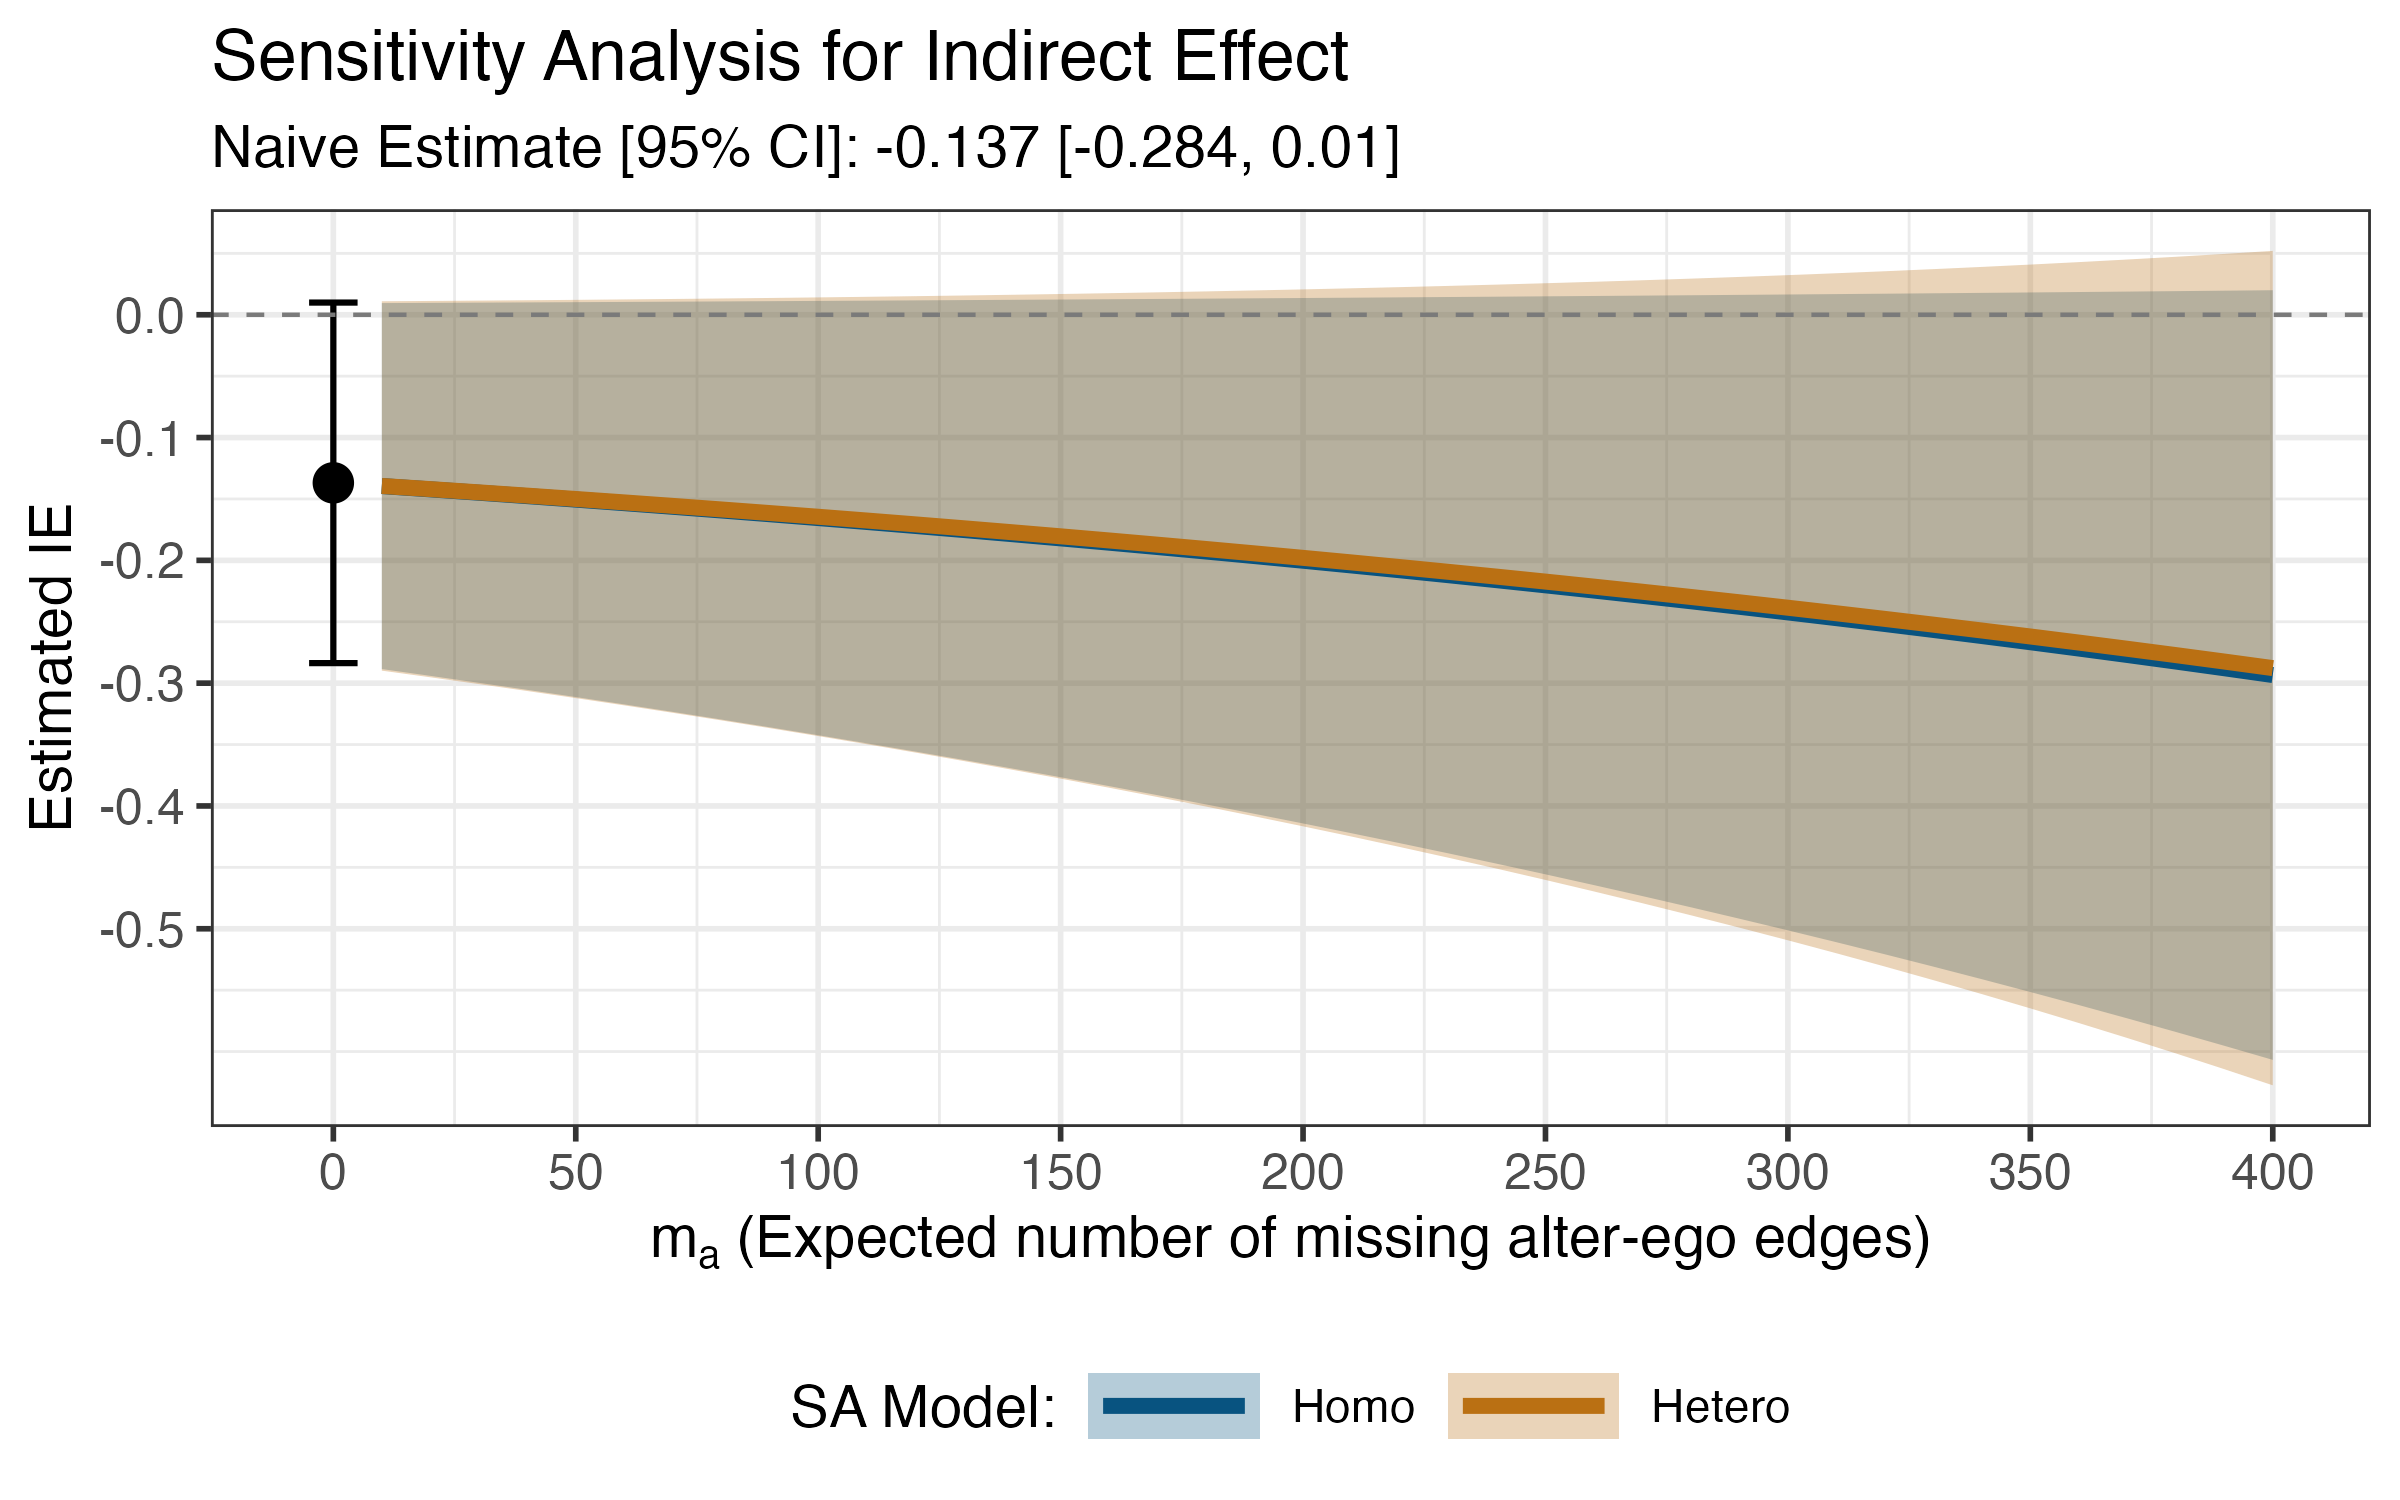
\includegraphics[width=0.7\linewidth]{figures/hptn/sa_ie_plot_not_augmented.png}
    \caption{Caption}
    \label{fig:hptn_sa_ie_augmented}
\end{figure}

\begin{figure}[H]
    \centering
    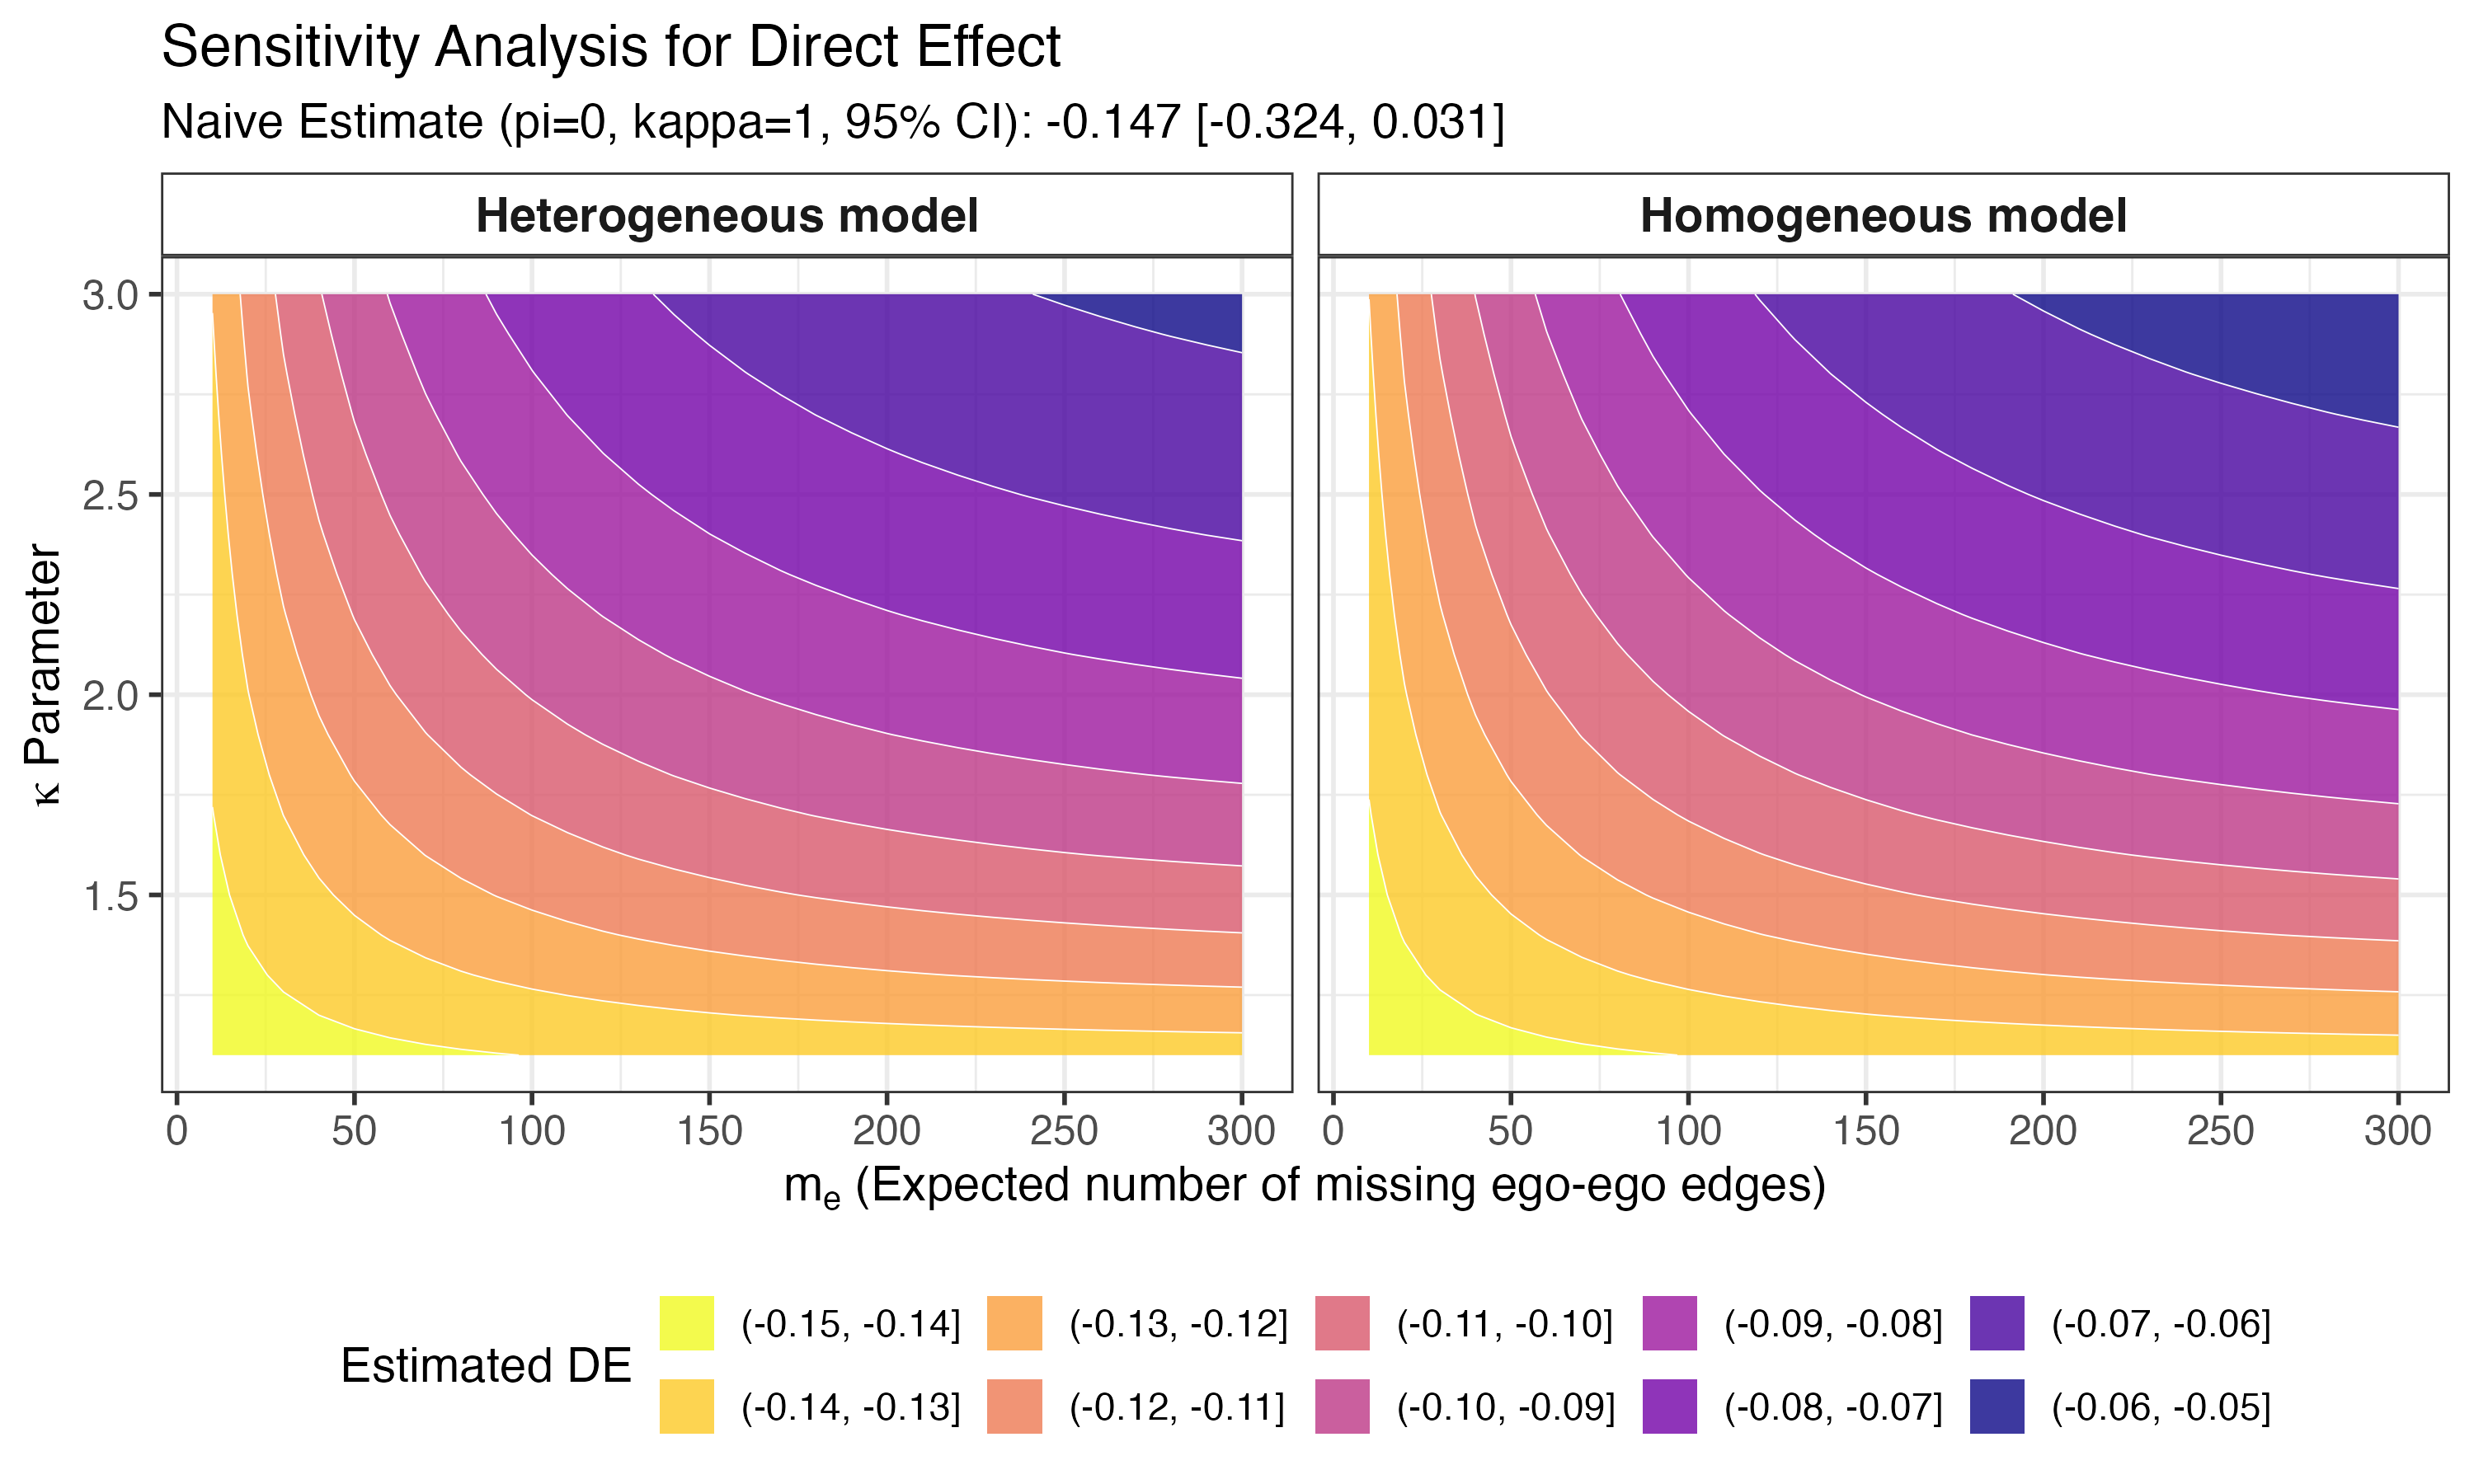
\includegraphics[width=0.8\linewidth]{figures/hptn/sa_de_plot.png}
    \caption{Caption}
    \label{fig:hptn_sa_de_augmented}
\end{figure}

\subsection{Probabilistic bias analysis}
\label{subsec:hptn_pba}

\begin{figure}[H]
    \centering
    
\includegraphics[width=0.6\linewidth]{figures/hptn/pba_ie_not_augmented.png}
    \caption{Caption}
    \label{fig:hptn_pba_ie_augmented}
\end{figure}

\begin{figure}[H]
    \centering
    
\includegraphics[width=0.6\linewidth]{figures/hptn/pba_de_not_augmented.png}
    \caption{Caption}
    \label{fig:hptn_pba_de_augmented}
\end{figure}

\section{Discussion}
\label{sec:discussion}

\begin{enumerate}
    \item In the case of homogeneous edge probabilities, it is possible to estimate $\pi^a_i$ (but not $\pi^e_i$) if we have validation data à la \citet{Chao2023}. They did it only for IE, and only on summary-level data.
    \item Extension to observational studies is tricky as non-recruited units can be treated as well... Discuss the limitations here.
    \item Possible extensions to CRTs (one-stage or two-stage randomization settings).
    \item Transporting the in-sample exposure-contrast estimand to population-level estimands will balance the tradeoff between the difficulty of data acquisition under interference (full population network is often required) and policy relevance.
\end{enumerate}

\bibliographystyle{apalike}
\bibliography{all_biblo}

\newpage

\appendix

\renewcommand{\theequation}{\thesection.\arabic{equation}}
\numberwithin{equation}{section}

\renewcommand\thefigure{\thesection.\arabic{figure}}    
\counterwithin{figure}{section}

\renewcommand\thetable{\thesection.\arabic{table}}    
\counterwithin{table}{section}

\section{Proofs}
\label{apdx_sec:proof}

\subsection{Indirect effects}

Recall that the HT estimator of the indirect effects based on the observed data \eqref{eq:IE_naive_HT} is
\begin{equation*}
    \widehat{IE} = 
    \frac{1}{n_a}
    \sum_{i \in \cR_a}
    \left[
    \frac{
    \mathbb{I}\{\widetilde{F}_i=1\}Y_i}{p_z} 
    -
    \frac{
    \mathbb{I}\{\widetilde{F}_i=0\}Y_i}{1 - p_z} 
    \right]
\end{equation*}
By the assumed experimental design (Assumption~\ref{ass:bernoulli_design}), the probability that an alter is assigned to treatment is zero, that is, $\Pr(Z_i =0 \mid i\in \cR_a)=0$. Also, $Z_i$ and $\widetilde{F}_i = F(\bZ_{-i},\widetilde{\bA})$ are independent. Thus, the event $\mathbb{I}\{\widetilde{F}_i=f\}$ is equal with probability one to  $\mathbb{I}\{Z_i=0,\widetilde{F}_i=f\}$ among the alters $i \in \cR_a$.
Starting with the first inner term, for $i \in \cR_a$,
\begin{equation}
    \label{apdx.eq:alter_0_1}
    \begin{aligned}        
    \EX_{\bZ}\left[\frac{
    \mathbb{I}\{\widetilde{F}_i=1\}Y_i}{p_z} \right]
    &\overset{(i)}{=}
     \frac{1}{p_z}
     \EX_{\bZ}
     \left[
    \mathbb{I}\{F_i=1,\widetilde{F}_i=1\}Y_i(0,1) 
    +
    \mathbb{I}\{F_i=0,\widetilde{F}_i=1\}Y_i(0,0) 
    \right]
    \\ &\overset{(ii)}{=}
    \frac{\Pr(F_i=1, \widetilde{F}_i=1 \mid i \in \cR_a)Y_i(0,1)}{p_z}
    \\ &\quad + 
    \frac{\Pr(F_i=0, \widetilde{F}_i=1 \mid i \in \cR_a)Y_i(0,0)}{p_z}
    \\ &\overset{(iii)}{=}
    \Pr(F_i = 1 \mid \widetilde{F}_i=1, i\in \cR_a) Y_i(0,1)
    \\ &\quad +
    \Pr(F_i = 0 \mid \widetilde{F}_i=1, i\in \cR_a) Y_i(0,0)
    \\ &\overset{(iv)}{=}
    Y_i(0,1),
    \end{aligned}
\end{equation}
where $(i)$ follows since $\mathbb{I}\{\widetilde{F}_i=f\}$ is equal with probability one to  $\mathbb{I}\{Z_i=0,\widetilde{F}_i=f\}$ and consistency (Assumption~\ref{ass:consis}) connect the observed outcomes $Y_i$ to the potential outcomes $Y_i(z,f)$; $(ii)$ from taking expectation with respect to the design $\bZ$; $(iii)$ since $p_z = \Pr(\widetilde{F}_i=1\mid i \in \cR_a)$ and $\frac{\Pr(F_i=f, \widetilde{F}_i=1 \mid i \in \cR_a)}{\Pr(\widetilde{F}_i=1\mid i \in \cR_a)} = \Pr(F_i = f \mid \widetilde{F}_i=1, i\in \cR_a)$; and $(iv)$ since $\Pr(F_i=1 \mid \widetilde{F}_i=1, i \in \cR_a) = 1$. To see this, note that $\sum_{j\neq i}\widetilde{A}_{ij}Z_j \leq \sum_{j\neq i}A_{ij}Z_j $ with probability one, which implies that $\widetilde{F}_i \leq F_i$ with probability one as well. Since $F_i$ is binary, if $\widetilde{F}_i=1$, it must also be $F_i=1$.
\\
\\ 
Moving to the second inner term, a similar derivation yields
\begin{align*}
     \EX_{\bZ}\left[\frac{
    \mathbb{I}\{\widetilde{F}_i=0\}Y_i}{1-p_z} \right]
    &= 
    \Pr(F_i = 1 \mid \widetilde{F}_i=0, i\in \cR_a) Y_i(0,1)
    \\ &\quad +
    \Pr(F_i = 0 \mid \widetilde{F}_i=0, i\in \cR_a) Y_i(0,0).
\end{align*}
By Bayes' rule, 
\begin{align*}
    \Pr(F_i = 0 \mid \widetilde{F}_i=0, i \in \cR_a)
    &= 
    \frac{\Pr(\widetilde{F}_i=0 \mid F_i=0, i \in \cR_a) \Pr(F_i=0 \mid i \in \cR_a)}
    {\Pr(\widetilde{F}_i=0 \mid i \in \cR_a)}
    \\ &= 
    \frac{\Pr(F_i=0 \mid i \in \cR_a)}
    {\Pr(\widetilde{F}_i=0 \mid i \in \cR_a)}
    \\ &=
    \frac{1-\pi^a_i}{1-p_z},
\end{align*}
as $\Pr(\widetilde{F}_i=0 \mid F_i=0, i \in \cR_a) = 1$ since $\widetilde{F}_i \leq F_i$ with probability one.
This yields
\begin{equation}
    \label{apdx.eq:alter_0_0}
     \EX_{\bZ}\left[\frac{
    \mathbb{I}\{\widetilde{F}_i=0\}Y_i}{1-p_z} \right]
    =
    \frac{\left(\pi_i^a -p_z\right)Y_i(0,1) + \left(1 - \pi_i^a\right)Y_i(0,0)}{1 - p_z}.
\end{equation}
Consequently, combining \eqref{apdx.eq:alter_0_1} and \eqref{apdx.eq:alter_0_0},
\begin{equation}
    \label{apdx.eq:alter_bias_ht}
    \begin{aligned}
        \EX_{\bZ}\left[\widehat{IE}\right]
        &= 
         \frac{1}{n_a}
    \sum_{i \in \cR_a}
    \left[
    Y_i(0,1)
    -
   \frac{\left(\pi_i^a -p_z\right)Y_i(0,1) + \left(1 - \pi_i^a\right)Y_i(0,0)}{1 - p_z}
    \right]
    \\ &=
    \frac{1}{n_a}
    \sum_{i \in \cR_a}
    \frac{1-\pi_i^a}{1-p_z}
    \left[
    Y_i(0,1) - Y_i(0,0)
    \right]
    \\ &=
    IE + \frac{1}{n_a}
    \sum_{i \in \cR_a}
    \frac{p_z-\pi_i^a}{1-p_z}
    \left[
    Y_i(0,1) - Y_i(0,0)
    \right],
    \end{aligned}
\end{equation}
which completes the proof of the first part of Proposition~\ref{prop:bias_naive_ht}.
\\
\\
The bias-corrected estimator is
\begin{equation*}
    \widehat{IE}_{adj} = 
    \frac{1}{n_a}
    \sum_{i \in \cR_a}
    \frac{1-p_z}{1-\pi_i^a}
    \left[
    \frac{
    \mathbb{I}\{\widetilde{F}_i=1\}Y_i}{p_z} 
    -
    \frac{
    \mathbb{I}\{\widetilde{F}_i=0\}Y_i}{1 - p_z} 
    \right].
\end{equation*}
As the weights $\frac{1-p_z}{1-\pi_i^a}$ are fixed and therefore independent of the design $\bZ$, taking the expectation $\EX_{\bZ}\left[\widehat{IE}_{adj}\right]$
will result in the second row of \eqref{apdx.eq:alter_bias_ht} where the terms $\frac{1-\pi_i^a}{1-p_z}$ and $\frac{1-p_z}{1-\pi_i^a}$ are multiplied and therefore canceled. That implies $\EX_{\bZ}\left[\widehat{IE}_{adj}\right]= IE$ and completes the proof of Proposition~\ref{prop:ie_sa}.

\paragraph{Variance estimation.} We derive variance estimators based on the augmented estimator \eqref{eq:IE_corrected_aipw}. Write
\begin{align*}
    \widehat{IE}_{adj}^{aug} &= 
    \frac{1}{n_a}
    \sum_{i \in \cR_a}
    \frac{1-p_z}{1-\pi_i^a}
    \left[
    \frac{
    \mathbb{I}\{
    \widetilde{F}_i=1\}\left(Y_i - m^a_i(1) \right)}{p_z} 
    -
    \frac{
    \mathbb{I}\{\widetilde{F}_i=0\}\left(Y_i - m^a_i(0) \right)}{1 - p_z} 
    + \left\{m^a_i(1) - m^a_i(0) \right\}
    \right]
    \\ &=
    \frac{1}{n_a}
    \sum_{i \in \cR_a}
    \frac{1-p_z}{1-\pi_i^a} \phi_i^a
    \\ &=
    \frac{1}{n_a}
    \sum_{i \in \cR_a}
    \alpha_i^a \phi_i^a,
\end{align*}
where $\alpha_i^a = \frac{1-p_z}{1-\pi_i^a}$.
We assume that the outcome models $m_i^a(f)$ are estimated through cross-fitting (\bwnote{TODO: add ref}) and therefore assumed to be independent of $\bZ$. We ignore the sampling uncertainty associated with estimating the outcome models. 

Alters in the same ego-network have the same observed exposure.
Recall that $e(i) \in \cR_e$ is the ego of alter $j \in \cR_a$.
We can write the adjusted IE estimator \eqref{eq:IE_corrected_aipw} as
\begin{equation*}
    \begin{aligned}
        \widehat{IE}_{adj}^{aug} &= 
        \frac{1}{n_a}
    \sum_{i \in \cR_a}
    \alpha_i^a \phi_i^a
    \\ &=
    \frac{1}{n_a}
    \sum_{i \in \cR_e}
    \sum_{j \in \cR_a : e(j)=i}
    \alpha_j^a \phi_j^a,
    \end{aligned}
\end{equation*}
which is the sum over all ego-networks of the sum of alters estimates within each ego-network.
As estimates of alters in the same ego-network are likely correlated (often represented as the intra-cluster correlation coefficient in cluster randomized trials),
we estimate the variance of $\widehat{IE}_{adj}^{aug}$ using the cluster-robust empirical variance estimator. For ego $i \in \cR_e$, write
\begin{equation*}
    T_i = \sum_{j \in \cR_a : e(j)=i}
    \alpha_j^a \phi_j^a,
\end{equation*}
such that 
\begin{equation*}
    \widehat{IE}_{adj}^{aug}=
     \frac{1}{n_a}
    \sum_{i \in \cR_e} T_i.
\end{equation*}
Let $\overline{T} = \frac{1}{n_e} \sum_{i \in \cR_e} T_i$.
Thus, $\widehat{IE}_{adj}^{aug} = \frac{n_e}{n_a} \overline{T}$. The cluster-robust empirical variance estimator is 
\begin{equation*}
    \widehat{Var}\left(\widehat{IE}_{adj}^{aug}\right)
    =
    \frac{n_e}{n_a^2(n_e-1)}
    \sum_{i \in \cR_e} 
    \left(
    T_i - \overline{T}
    \right)^2.
\end{equation*}
Alternatively, it is also possible to estimate the variance of $\widehat{IE}_{adj}^{aug}$ by nonparametric network bootstrap, where we resample ego-networks.



\paragraph{Attenuation towards the null.}
Eq.~\eqref{eq:pi_a} implies that $\pi^a_i \geq p_z$, therefore $\frac{1-p_z}{1-\pi^a_i} \geq 1$.
If $\pi^a_i = \pi^a$ for all $i\in\cR_a$, that is, the same for all alters, then $\widehat{IE}_{adj}=\frac{1-p_z}{1-\pi^a}\widehat{IE}$. Thus, $\text{sign}(\widehat{IE}_{adj})=\text{sign}(\widehat{IE})$ and 
\begin{align*}
    \begin{cases}
        \widehat{IE}_{adj} \geq \widehat{IE}, & \widehat{IE} > 0, \\
        \widehat{IE}_{adj} \leq \widehat{IE}, & \widehat{IE} < 0.
    \end{cases}
\end{align*}
Moreover, if $Y_i(0,1) \geq Y_i(0,0)$ for all $i \in \cR_a$ such that $IE\geq0$, then since $p_z - \pi_i^a \leq 0$, from \eqref{apdx.eq:alter_bias_ht}, we have $\EX_{\bZ}\left[\widehat{IE}\right] \leq IE$. Vice versa, if $Y_i(0,1) \leq Y_i(0,0)$ for all $i \in \cR_a$, then $IE \leq 0$ and $\EX_{\bZ}\left[\widehat{IE}\right] \geq IE$. That is, the estimator $\widehat{IE}$ is, in expectation, attenuated towards the null of no indirect effects.

\paragraph{Exposure probabilities of alters.}
For alters $i\in\cR_a$, $F_i=1$ if its ego $e(i)$ or at least one of the other recruited egos connected to $i$ in the population network $\bA$ is treated. We have
\begin{align*}
    \pi^a_i &= \Pr(F_i=1 \mid i\in \cR_a) 
    \\ &=
    \Pr(F_i=1 \mid Z_{e(i)}=1, i\in \cR_a)\Pr(Z_{e(i)}=1\mid i \in \cR_a) 
    \\ &\quad + \Pr(F_i=1 \mid Z_{e(i)}=0, i\in \cR_a)\Pr(Z_{e(i)}=0\mid i \in \cR_a),
\end{align*}
but $\Pr(F_i=1 \mid Z_{e(i)}=1, i\in \cR_a)=1$ and $\Pr(Z_{e(i)}=1\mid i \in \cR_a)=p_z 1\{e(i) \in \cR_e\}$ by Assumptions~\ref{ass:bernoulli_design} and \ref{ass:expos_map}. Since only recruited egos have a non-zero probability of being assigned to treatment, then for alter $i\in \cR_a$, $F_i = \sum_{j\neq i}Z_jA_{ij}=\sum_{j \in \cR_e}Z_jA_{ij}$ with probability one. Thus, $F_i = 0 \mid  Z_{e(i)}=0, i\in \cR_a$ equal with probability one to $1\{\sum_{j \in \cR_e \setminus e(i)}Z_jA_{ij}=0\}$. Thus,
\begin{align*}
    \Pr(F_i=0 \mid Z_{e(i)}=0, i\in \cR_a) =
    \prod_{j \in  \cR_e \setminus \{e(i)\}}
    \big(1 - p_z \rho^a_{ij}\big),
\end{align*}
which yield \eqref{eq:pi_a}.

\paragraph{Extension to relative risk estimand and estimators.}
In the case of binary outcomes, we can also consider the relative risk (RR) estimand
\begin{equation}
    \label{apdx.eq:IE_ratio}
    IE^{RR} = \frac{
    \sum_{i \in \cR_a}Y_i(0,1)}{
    \sum_{i \in \cR_a}Y_i(0,0)
    }.
\end{equation}
Analogously to \eqref{eq:IE_naive_HT}, the estimator based on the observed data is therefore
\begin{equation}
    \label{apdx.eq:ie_ratio_ht}
    \widehat{IE}^{RR} =
    \frac{
    \sum_{i \in \cR_a}\frac{
    \mathbb{I}\{\widetilde{F}_i=1\}Y_i}{p_z}}{
    \sum_{i \in \cR_a}\frac{
    \mathbb{I}\{\widetilde{F}_i=0\}Y_i}{1 - p_z}
    }.
\end{equation}
We saw in \eqref{apdx.eq:alter_0_1} that the numerator in \eqref{apdx.eq:ie_ratio_ht} is an unbiased estimator of the numerator in \eqref{apdx.eq:IE_ratio}.
However, from \eqref{apdx.eq:alter_0_0} the denominator is biased. Rearranging \eqref{apdx.eq:alter_0_0}, 
\begin{equation*}
      \frac{1-p_z}{1-\pi_i^a}\EX_{\bZ}\left[\frac{
    \mathbb{I}\{\widetilde{F}_i=0\}Y_i}{1-p_z} \right]
    =
    Y_i(0,0) +
    \frac{\pi_i^a - p_z}{1-\pi_i^a}Y_i(0,1).
\end{equation*}
Thus, using \eqref{apdx.eq:alter_0_1}, we can unbiasedly estimate $Y_i(0,0)$ through
\begin{equation*}
     \frac{1-p_z}{1-\pi_i^a}
     \frac{
    \mathbb{I}\{\widetilde{F}_i=0\}Y_i}{1-p_z} -
     \frac{\pi_i^a - p_z}{1-\pi_i^a} \frac{
    \mathbb{I}\{\widetilde{F}_i=1\}Y_i}{p_z}.
\end{equation*}
That motivates the adjusted estimator
\begin{equation}
    \label{apdx.eq:IE_ratio_adjusted_esti}
    \widehat{IE}^{RR}_{adj} =
    \frac{
    \sum_{i \in \cR_a}\frac{
    \mathbb{I}\{\widetilde{F}_i=1\}Y_i}{p_z}}{
    \sum_{i \in \cR_a}\frac{1-p_z}{1-\pi_i^a}
     \frac{
    \mathbb{I}\{\widetilde{F}_i=0\}Y_i}{1-p_z} -
     \frac{\pi_i^a - p_z}{1-\pi_i^a} \frac{
    \mathbb{I}\{\widetilde{F}_i=1\}Y_i}{p_z}
    }.
\end{equation}
Being a ratio estimator, \eqref{apdx.eq:IE_ratio_adjusted_esti} is biased, but the bias can be easily bounded \citep{Saerndal2003}.

\subsection{Direct effects}

Recall that the HT estimator of direct effects based on the observed data \eqref{eq:DE_naive_HT} is
\begin{equation*}
    \widehat{DE} = 
    \frac{1}{n_e}
    \sum_{i \in \cR_e}
    \left[
    \frac{
    \mathbb{I}\{Z_i=1\}Y_i}{p_z} 
    -
    \frac{
    \mathbb{I}\{Z_i=0\}Y_i}{1 - p_z} 
    \right].
\end{equation*}
Also, the observed exposure of all egos is zero $\Pr(\widetilde{F}_i =0 \mid i \in \cR_e) =1$. By the assumed expermential design (Assumption~\ref{ass:bernoulli_design}), the event $\mathbb{I}\{Z_i=z\}$ is equal with probability one to $\mathbb{I}\{Z_i=z, \widetilde{F}_i =0\}$ among the egos $i \in \cR_e$.
The expectation of the first inner term of $\widehat{DE}$, for $i \in \cR_e$, is as follows.
\begin{equation*}
    % \label{apdx.eq:egos_z_0}
    \begin{aligned}        
    \EX_{\bZ}\left[\frac{
    \mathbb{I}\{Z_i=1\}Y_i}{p_z} \right]
    &\overset{(i)}{=}
    \EX_{\bZ}\left[\frac{
    \mathbb{I}\{Z_i=1, \widetilde{F}_i =0\}Y_i}{p_z} \right]
    \\ &\overset{(ii)}{=}
     \frac{1}{p_z}
     \EX_{\bZ}
     \left[
    \mathbb{I}\{Z_i=1,F_i=1,\widetilde{F}_i=0\}Y_i(1,1) 
    \right]
    \\ &\quad +
    \frac{1}{p_z}
     \EX_{\bZ}
     \left[
    \mathbb{I}\{Z_i=1,F_i=0,\widetilde{F}_i=0\}Y_i(0,0) 
    \right]
    \\ &\overset{(iii)}{=}
    \Pr(F_i=1, \widetilde{F}_i=0 \mid i \in \cR_e)Y_i(1,1)
    \\ &\quad + 
    \Pr(F_i=0, \widetilde{F}_i=0 \mid i \in \cR_e)Y_i(1,0)
    \\ &\overset{(iv)}{=}
     \frac{\Pr(F_i=1, \widetilde{F}_i=0 \mid i \in \cR_e)}{\Pr(\widetilde{F}_i=0 \mid i\in \cR_e)}Y_i(1,1)
    \\ &\quad + 
    \frac{\Pr(F_i=0, \widetilde{F}_i=0 \mid i \in \cR_e)}{\Pr(\widetilde{F}_i=0 \mid i\in \cR_e)}
    Y_i(1,0)
    \\ &=
    \Pr(F_i=0 \mid \widetilde{F}_i=0, i \in \cR_e)
    Y_i(1,1)
    \\ &\quad +
    \Pr(F_i=1 \mid \widetilde{F}_i=0, i \in \cR_e)
    Y_i(1,0),
    \end{aligned}
\end{equation*}
where $(i)$ follows from the explanation described above; $(ii)$ from consistency (Assumption~\ref{ass:consis});
$(iii)$ since $Z_i$ is independent from both $F_i$ and $\widetilde{F}_i$ by Assumption~\ref{ass:bernoulli_design}, and $\Pr(Z_i=1\mid i \in \cR_e)=p_z$; and $(iv)$ since $\Pr(\widetilde{F}_i=0 \mid i\in \cR_e)=1$.
By Bayes' rule, 
\begin{align*}
    \Pr(F_i =1 \mid \widetilde{F}_i=0, i \in \cR_e) &=
    \frac{\Pr(\widetilde{F}_i=0 \mid F_i=1, i \in \cR_e) \Pr(F_i=1 \mid i \in \cR_e)}
    {\Pr(\widetilde{F}_i=0 \mid i \in \cR_e)}
    \\ &= \Pr(F_i=1 \mid i \in \cR_e),
\end{align*}
since $\widetilde{F}_i = 0$ with probability one for $i\in \cR_e$, which implies that 
$\Pr(\widetilde{F}_i=0 \mid i \in \cR_e)$ and the conditional probability
$\Pr(\widetilde{F}_i=0 \mid F_i = f ,i \in \cR_e)$ equal to one.
Let $\pi^e_i = \Pr(F_i =1 \mid i \in \cR_e)$. 
Plugging this into the above expectation yields 
\begin{equation}
    \label{apdx.eq:ego_1_0}
    \EX_{\bZ}\left[\frac{
    \mathbb{I}\{Z_i=1\}Y_i}{p_z} \right]
    = \pi_i^e Y_i(1,1) + (1-\pi_i^e)Y_i(1,0).
    \end{equation}
Similarly, for $z=0$ we have
\begin{equation}
    \label{apdx.eq:ego_0_0}
    \EX_{\bZ}\left[\frac{
    \mathbb{I}\{Z_i=0\}Y_i}{1-p_z} \right]
    = \pi_i^e Y_i(0,1) + (1-\pi_i^e)Y_i(0,0).
    \end{equation}
Plugging \eqref{apdx.eq:ego_1_0} and \eqref{apdx.eq:ego_0_0} into $\EX_{\bZ}\left[\widehat{DE}\right]$ yields
\begin{equation}
    \label{apdx.eq:ego_ht_bias}
    \begin{aligned}
    \EX_{\bZ}\left[\widehat{DE}\right]
    &=
     \frac{1}{n_e}
    \sum_{i \in \cR_e}
    \left[
    \pi_i^e\left\{Y_i(1,1) - Y_i(0,1)
    \right\}
    +
    (1-\pi_i^e)\left\{Y_i(1,0) - Y_i(0,0)
    \right\}
    \right]
    \\ &=
    DE + 
    \frac{1}{n_e} 
    \sum_{i\in\cR_e}
    \pi_i^e
    \left[
    \left\{ Y_i(1, 1) - Y_i(0,1)\right\} 
    - \left \{ Y_i(1,0) - Y_i(0,0) \right\}
    \right],
    \end{aligned}
\end{equation}
which completes the second part of Proposition~\ref{prop:bias_naive_ht}.
\\
\\
Now, under Assumption~\ref{ass:egos_kappa}, $Y_i(1,1)-Y_i(0,1) = \kappa \left\{Y_i(1,0) - Y_i(0,0) \right\}$. Recall that the adjusted DE estimator \eqref{eq:DE_corrected} is 
\begin{equation*}
       \widehat{DE}_{adj} =
    \frac{1}{n_e}
    \sum_{i \in \cR_e}
    \frac{1}{1 + \pi_i^e(\kappa-1)}
    \left[
    \frac{
    \mathbb{I}\{Z_i=1\}Y_i}{p_z} 
    -
    \frac{
    \mathbb{I}\{Z_i=0\}Y_i}{1 - p_z} 
    \right].
\end{equation*}
Since both $\kappa$ and $\pi_i^e$ are fixed and therefore independent of $\bZ$, we can use \eqref{apdx.eq:ego_1_0}, \eqref{apdx.eq:ego_0_0}, and \eqref{apdx.eq:ego_ht_bias} to obtain
\begin{equation*}
    \begin{aligned}
        \EX \left[\widehat{DE}_{adj} \right]
        &=
        \frac{1}{n_e}
    \sum_{i \in \cR_e}
    \frac{1}{1 + \pi_i^e(\kappa-1)}
    \left[
    \pi_i^e\left\{Y_i(1,1) - Y_i(0,1)
    \right\}
    +
    (1-\pi_i^e)\left\{Y_i(1,0) - Y_i(0,0)
    \right\}
    \right]
    \\ &\overset{(i)}{=}
      \frac{1}{n_e}
    \sum_{i \in \cR_e}
    \frac{1}{1 + \pi_i^e(\kappa-1)}
    \left[
    \pi_i^e\kappa\left\{Y_i(1,0) - Y_i(0,0)
    \right\}
    +
    (1-\pi_i^e)\left\{Y_i(1,0) - Y_i(0,0)
    \right\}
    \right]
    \\ &=
    \frac{1}{n_e}
    \sum_{i \in \cR_e}
    Y_i(1,0) - Y_i(0,0)
    \\ &=
    DE,
    \end{aligned}
\end{equation*}
where in $(i)$ we used Assumption~\ref{ass:egos_kappa}.

\paragraph{Variance estimation.} We derive variance estimators based on the augmented estimator \eqref{eq:DE_corrected_aipw}. 
Write
\begin{align*}
    \widehat{DE}_{adj}^{aug} 
        &= 
    \frac{1}{n_e}
    \sum_{i \in \cR_e}
    \frac{1}{1 + \pi_i^e(\kappa-1)}
    \left[
    \frac{
    \mathbb{I}\{
    Z_i=1\}\left(Y_i - m^e_i(1) \right)}{p_z} 
    -
    \frac{
    \mathbb{I}\{Z_i=0\}\left(Y_i - m^e_i(0) \right)}{1 - p_z} 
    + \left\{m^e_i(1) - m^e_i(0) \right\}
    \right],
    \\ &=
    \frac{1}{n_a}
    \sum_{i \in \cR_a}
    \frac{1}{1 + \pi_i^e(\kappa-1)} \phi_i^e
    \\ &=
    \frac{1}{n_a}
    \sum_{i \in \cR_a}
    \alpha_i^e \phi_i^e.
\end{align*}
We assume that the outcome models $m_i^e(z)$ are estimated through cross-fitting (\bwnote{TODO: add ref}) and therefore assumed to be independent of $\bZ$. We ignore the sampling uncertainty associated with estimating the outcome models. 
We estimate the variance using the empirical estimate
\begin{equation*}
    \begin{aligned}
        \widehat{Var}\left(\widehat{DE}_{adj}^{aug}\right)
        &= 
        \frac{1}{n_e(n_e-1)}
        \sum_{i\in \cR_e}
        \left(
        \alpha_i^e \phi_i^e 
        -
        \frac{1}{n_a}
    \sum_{i \in \cR_a}
    \alpha_i^e \phi_i^e
        \right)^2
        \\ &=
        \frac{1}{n_e(n_e-1)}
        \sum_{i\in \cR_e}
        \left(
        \alpha_i^e \phi_i^e 
        -
       \widehat{DE}_{adj}^{aug}
        \right)^2.
    \end{aligned}
\end{equation*}
Alternatively, it is also possible to estimate the variance of $\widehat{DE}_{adj}^{aug}$ by nonparametric network bootstrap, where we resample ego-networks.

\paragraph{Interplay between $\kappa$ and $\pi_i^e$.}
\bwnote{TODO: write about the adjusted DE estimator compared to the naive one in terms of $\kappa$ and $\pi_i^e$ combinations.}

\section{Simulations}

{\renewcommand{\arraystretch}{0.8} % Shrink row height to 80% (adjust 0.8 as needed)

\begin{table}[H]

\caption{IE Results - Heterogeneous Exposure - not aug}
\centering
\begin{tabular}[t]{lccccc}
\toprule
Scenario & spec & Variance & bias & coverage & ese\_ase\\
\midrule
 &  & Analytic & 0.016 & 0.972 & 0.855\\
\cmidrule{3-6}
 & \multirow{-2}{*}{\centering\arraybackslash Heterogeneous} & Bootstrap & 0.016 & 0.972 & 0.857\\
\cmidrule{2-6}
 &  & Analytic & 0.015 & 0.973 & 0.855\\
\cmidrule{3-6}
 & \multirow{-2}{*}{\centering\arraybackslash Homogeneous} & Bootstrap & 0.015 & 0.972 & 0.857\\
\cmidrule{2-6}
 &  & Analytic & -0.029 & 0.943 & 0.855\\
\cmidrule{3-6}
\multirow{-6}{*}[1\dimexpr\aboverulesep+\belowrulesep+\cmidrulewidth]{\raggedright\arraybackslash $m_a=100, IE=0.358$} & \multirow{-2}{*}{\centering\arraybackslash Naive} & Bootstrap & -0.029 & 0.943 & 0.857\\
\cmidrule{1-6}
 &  & Analytic & 0.006 & 0.974 & 0.872\\
\cmidrule{3-6}
 & \multirow{-2}{*}{\centering\arraybackslash Heterogeneous} & Bootstrap & 0.006 & 0.972 & 0.874\\
\cmidrule{2-6}
 &  & Analytic & 0.008 & 0.975 & 0.867\\
\cmidrule{3-6}
 & \multirow{-2}{*}{\centering\arraybackslash Homogeneous} & Bootstrap & 0.008 & 0.974 & 0.869\\
\cmidrule{2-6}
 &  & Analytic & -0.068 & 0.831 & 0.867\\
\cmidrule{3-6}
\multirow{-6}{*}[1\dimexpr\aboverulesep+\belowrulesep+\cmidrulewidth]{\raggedright\arraybackslash $m_a=200, IE=0.335$} & \multirow{-2}{*}{\centering\arraybackslash Naive} & Bootstrap & -0.068 & 0.829 & 0.869\\
\cmidrule{1-6}
 &  & Analytic & -0.003 & 0.975 & 0.871\\
\cmidrule{3-6}
 & \multirow{-2}{*}{\centering\arraybackslash Heterogeneous} & Bootstrap & -0.003 & 0.975 & 0.873\\
\cmidrule{2-6}
 &  & Analytic & 0.003 & 0.975 & 0.872\\
\cmidrule{3-6}
 & \multirow{-2}{*}{\centering\arraybackslash Homogeneous} & Bootstrap & 0.003 & 0.975 & 0.874\\
\cmidrule{2-6}
 &  & Analytic & -0.097 & 0.697 & 0.872\\
\cmidrule{3-6}
\multirow{-6}{*}[1\dimexpr\aboverulesep+\belowrulesep+\cmidrulewidth]{\raggedright\arraybackslash $m_a=300, IE=0.318$} & \multirow{-2}{*}{\centering\arraybackslash Naive} & Bootstrap & -0.097 & 0.696 & 0.874\\
\bottomrule
\end{tabular}
\end{table}
}

{\renewcommand{\arraystretch}{0.8} 

\begin{table}[H]

\caption{DE Results - Heterogeneous Exposure - not aug}
\centering
\begin{tabular}[t]{lccccc}
\toprule
Scenario & spec & Variance & bias & coverage & ese\_ase\\
\midrule
 &  & Analytic & 0.014 & 0.950 & 0.968\\
\cmidrule{3-6}
 & \multirow{-2}{*}{\centering\arraybackslash Heterogeneous} & Bootstrap & 0.014 & 0.950 & 0.970\\
\cmidrule{2-6}
 &  & Analytic & 0.011 & 0.950 & 0.972\\
\cmidrule{3-6}
 & \multirow{-2}{*}{\centering\arraybackslash Homogeneous} & Bootstrap & 0.011 & 0.949 & 0.975\\
\cmidrule{2-6}
 &  & Analytic & 0.090 & 0.776 & 0.972\\
\cmidrule{3-6}
\multirow{-6}{*}[1\dimexpr\aboverulesep+\belowrulesep+\cmidrulewidth]{\raggedright\arraybackslash $m_e=50, DE=0.345$} & \multirow{-2}{*}{\centering\arraybackslash Naive} & Bootstrap & 0.090 & 0.773 & 0.975\\
\cmidrule{1-6}
 &  & Analytic & 0.017 & 0.932 & 1.035\\
\cmidrule{3-6}
 & \multirow{-2}{*}{\centering\arraybackslash Heterogeneous} & Bootstrap & 0.017 & 0.931 & 1.038\\
\cmidrule{2-6}
 &  & Analytic & 0.016 & 0.932 & 1.042\\
\cmidrule{3-6}
 & \multirow{-2}{*}{\centering\arraybackslash Homogeneous} & Bootstrap & 0.016 & 0.933 & 1.045\\
\cmidrule{2-6}
 &  & Analytic & 0.212 & 0.249 & 1.042\\
\cmidrule{3-6}
\multirow{-6}{*}[1\dimexpr\aboverulesep+\belowrulesep+\cmidrulewidth]{\raggedright\arraybackslash $m_e=150, DE=0.355$} & \multirow{-2}{*}{\centering\arraybackslash Naive} & Bootstrap & 0.212 & 0.250 & 1.045\\
\cmidrule{1-6}
 &  & Analytic & 0.015 & 0.944 & 0.985\\
\cmidrule{3-6}
 & \multirow{-2}{*}{\centering\arraybackslash Heterogeneous} & Bootstrap & 0.015 & 0.942 & 0.988\\
\cmidrule{2-6}
 &  & Analytic & 0.014 & 0.940 & 0.988\\
\cmidrule{3-6}
 & \multirow{-2}{*}{\centering\arraybackslash Homogeneous} & Bootstrap & 0.014 & 0.940 & 0.991\\
\cmidrule{2-6}
 &  & Analytic & 0.271 & 0.109 & 0.988\\
\cmidrule{3-6}
\multirow{-6}{*}[1\dimexpr\aboverulesep+\belowrulesep+\cmidrulewidth]{\raggedright\arraybackslash $m_e=250, DE=0.345$} & \multirow{-2}{*}{\centering\arraybackslash Naive} & Bootstrap & 0.271 & 0.108 & 0.991\\
\bottomrule
\end{tabular}
\end{table}
}

{\renewcommand{\arraystretch}{0.8} 

\begin{table}[H]

\caption{IE Results - homogeneous Exposure - Augmented}
\centering
\begin{tabular}[t]{lccccc}
\toprule
Scenario & spec & Variance & bias & coverage & ese\_ase\\
\midrule
 &  & Analytic & 0.010 & 0.987 & 0.741\\
\cmidrule{3-6}
 & \multirow{-2}{*}{\centering\arraybackslash Heterogeneous} & Bootstrap & 0.010 & 0.988 & 0.740\\
\cmidrule{2-6}
 &  & Analytic & 0.009 & 0.988 & 0.742\\
\cmidrule{3-6}
 & \multirow{-2}{*}{\centering\arraybackslash Homogeneous} & Bootstrap & 0.009 & 0.987 & 0.745\\
\cmidrule{2-6}
 &  & Analytic & -0.035 & 0.943 & 0.743\\
\cmidrule{3-6}
\multirow{-6}{*}[1\dimexpr\aboverulesep+\belowrulesep+\cmidrulewidth]{\raggedright\arraybackslash $m_a=100, IE=0.362$} & \multirow{-2}{*}{\centering\arraybackslash Naive} & Bootstrap & -0.035 & 0.942 & 0.741\\
\cmidrule{1-6}
 &  & Analytic & -0.002 & 0.976 & 0.867\\
\cmidrule{3-6}
 & \multirow{-2}{*}{\centering\arraybackslash Heterogeneous} & Bootstrap & -0.002 & 0.975 & 0.870\\
\cmidrule{2-6}
 &  & Analytic & -0.001 & 0.977 & 0.865\\
\cmidrule{3-6}
 & \multirow{-2}{*}{\centering\arraybackslash Homogeneous} & Bootstrap & -0.001 & 0.976 & 0.864\\
\cmidrule{2-6}
 &  & Analytic & -0.072 & 0.681 & 0.864\\
\cmidrule{3-6}
\multirow{-6}{*}[1\dimexpr\aboverulesep+\belowrulesep+\cmidrulewidth]{\raggedright\arraybackslash $m_a=200, IE=0.32$} & \multirow{-2}{*}{\centering\arraybackslash Naive} & Bootstrap & -0.071 & 0.678 & 0.864\\
\cmidrule{1-6}
 &  & Analytic & -0.039 & 0.949 & 0.860\\
\cmidrule{3-6}
 & \multirow{-2}{*}{\centering\arraybackslash Heterogeneous} & Bootstrap & -0.039 & 0.949 & 0.861\\
\cmidrule{2-6}
 &  & Analytic & -0.046 & 0.931 & 0.861\\
\cmidrule{3-6}
 & \multirow{-2}{*}{\centering\arraybackslash Homogeneous} & Bootstrap & -0.046 & 0.931 & 0.863\\
\cmidrule{2-6}
 &  & Analytic & -0.148 & 0.076 & 0.864\\
\cmidrule{3-6}
\multirow{-6}{*}[1\dimexpr\aboverulesep+\belowrulesep+\cmidrulewidth]{\raggedright\arraybackslash $m_a=300, IE=0.372$} & \multirow{-2}{*}{\centering\arraybackslash Naive} & Bootstrap & -0.148 & 0.075 & 0.864\\
\bottomrule
\end{tabular}
\end{table}
}

{\renewcommand{\arraystretch}{0.8} 

\begin{table}[H]

\caption{DE Results - homogeneous Exposure - Augmented}
\centering
\begin{tabular}[t]{lccccc}
\toprule
Scenario & spec & Variance & bias & coverage & ese\_ase\\
\midrule
 &  & Analytic & 0.021 & 0.953 & 0.887\\
\cmidrule{3-6}
 & \multirow{-2}{*}{\centering\arraybackslash Heterogeneous} & Bootstrap & 0.021 & 0.954 & 0.887\\
\cmidrule{2-6}
 &  & Analytic & 0.019 & 0.955 & 0.882\\
\cmidrule{3-6}
 & \multirow{-2}{*}{\centering\arraybackslash Homogeneous} & Bootstrap & 0.019 & 0.955 & 0.885\\
\cmidrule{2-6}
 &  & Analytic & 0.094 & 0.666 & 0.884\\
\cmidrule{3-6}
\multirow{-6}{*}[1\dimexpr\aboverulesep+\belowrulesep+\cmidrulewidth]{\raggedright\arraybackslash $m_e=50, DE=0.32$} & \multirow{-2}{*}{\centering\arraybackslash Naive} & Bootstrap & 0.094 & 0.664 & 0.885\\
\cmidrule{1-6}
 &  & Analytic & 0.093 & 0.297 & 0.943\\
\cmidrule{3-6}
 & \multirow{-2}{*}{\centering\arraybackslash Heterogeneous} & Bootstrap & 0.094 & 0.303 & 0.950\\
\cmidrule{2-6}
 &  & Analytic & 0.088 & 0.333 & 0.957\\
\cmidrule{3-6}
 & \multirow{-2}{*}{\centering\arraybackslash Homogeneous} & Bootstrap & 0.088 & 0.332 & 0.958\\
\cmidrule{2-6}
 &  & Analytic & 0.290 & 0.002 & 0.956\\
\cmidrule{3-6}
\multirow{-6}{*}[1\dimexpr\aboverulesep+\belowrulesep+\cmidrulewidth]{\raggedright\arraybackslash $m_e=150, DE=0.295$} & \multirow{-2}{*}{\centering\arraybackslash Naive} & Bootstrap & 0.290 & 0.001 & 0.957\\
\cmidrule{1-6}
 &  & Analytic & -0.027 & 0.913 & 0.918\\
\cmidrule{3-6}
 & \multirow{-2}{*}{\centering\arraybackslash Heterogeneous} & Bootstrap & -0.027 & 0.910 & 0.920\\
\cmidrule{2-6}
 &  & Analytic & -0.032 & 0.873 & 0.911\\
\cmidrule{3-6}
 & \multirow{-2}{*}{\centering\arraybackslash Homogeneous} & Bootstrap & -0.032 & 0.877 & 0.912\\
\cmidrule{2-6}
 &  & Analytic & 0.216 & 0.024 & 0.909\\
\cmidrule{3-6}
\multirow{-6}{*}[1\dimexpr\aboverulesep+\belowrulesep+\cmidrulewidth]{\raggedright\arraybackslash $m_e=250, DE=0.38$} & \multirow{-2}{*}{\centering\arraybackslash Naive} & Bootstrap & 0.217 & 0.026 & 0.909\\
\bottomrule
\end{tabular}
\end{table}
}

\section{Data analysis}

\begin{figure}[H]
    \centering
    
\includegraphics[width=0.6\linewidth]{figures/hptn/alter_per_egonet_histogram.png}
    \caption{Caption}
    \label{fig:hptn_degree}
\end{figure}

\begin{figure}[H]
    \centering
    
\includegraphics[width=0.7\linewidth]{figures/hptn/sa_de_plot_aug_kappa2.png}
    \caption{Caption}
    \label{fig:sa_de_kappa2}
\end{figure}

\end{document}
